% define document type (i.e., template. Here: A4 APA manuscript with 12pt font)
\documentclass[man, 12pt, a4paper, mask]{apa7}

% change margins (e.g., for margin comments):
%\usepackage{geometry}
% \geometry{
% a4paper,
% marginparwidth=30mm,
% right=50mm,
%}

% add packages
\usepackage[american]{babel}
\usepackage[utf8]{inputenc}
\usepackage{csquotes}
\usepackage{hyperref}
\usepackage[style=apa, sortcites=true, sorting=nyt, backend=biber, natbib=true, uniquename=false, uniquelist=false, useprefix=true]{biblatex}
\usepackage{authblk}
\usepackage{graphicx}
\usepackage{setspace,caption}
\usepackage{subcaption}
\usepackage{enumitem}
\usepackage{lipsum}
\usepackage{soul}
\usepackage{xcolor}
\usepackage{fourier}
\usepackage{stackengine}
\usepackage{scalerel}
\usepackage{fontawesome5}
\usepackage[normalem]{ulem}
% \usepackage{longtable}
\usepackage{amsmath, nccmath}
\usepackage{mdframed}
\usepackage{ntheorem}
\usepackage{afterpage}
\usepackage{float}
\usepackage{array}
\usepackage{censor}
\usepackage{pdflscape}
\usepackage{lscape}
\usepackage{pdfpages}
\usepackage{enumitem}
\usepackage{caption}
\usepackage{adjustbox}
\usepackage{makecell}
\usepackage{tabu}
% Path Diagrams
\usepackage{tikz}
\usepackage{pgfplots}
\pgfplotsset{compat=1.17}
\tikzset{mynode/.style={draw,text width=1in,align=center} }
\usetikzlibrary{positioning}

% make warning with red triangle
\newcommand\Warning[1][2ex]{%
  \renewcommand\stacktype{L}%
  \scaleto{\stackon[1.3pt]{\color{red}$\triangle$}{\tiny\bfseries !}}{#1}}%

% make question with red triangle
\newcommand\Question[1][2ex]{%
  \renewcommand\stacktype{L}%
  \scaleto{\stackon[1.3pt]{\color{red}$\triangle$}{\tiny\bfseries ?}}{#1}}%
  
% add definition sections
\theoremstyle{break}
\newtheorem{definition}{Definition}

% add hypothesis sections
\theoremstyle{plain}
\theoremseparator{:}
\newtheorem{hyp}{Hypothesis}

\newtheorem{subhyp}{Hypothesis}
   \renewcommand\thesubhyp{\thehyp\alph{subhyp}}

% Analysis Plan sections (probably better as Definitions or Remarks instead of Theorems)
\newtheorem{ap}{Hypothesis}

\newtheorem{subap}{Hypothesis}
   \renewcommand\thesubap{\theap\alph{subap}}

% add quote section
\usepackage{csquotes}

% framed box section
\usepackage{framed}
\emergencystretch=1em

% formatting links in the PDF file
\hypersetup{
pdfpagemode={UseOutlines},
bookmarksopen=true,
bookmarksopenlevel=0,
hypertexnames=false,
colorlinks   = true, %Colours links instead of ugly boxes
urlcolor     = blue, %Colour for external hyperlinks
linkcolor    = blue, %Colour of internal links
citecolor   = cyan, %Colour of citations
pdfstartview={FitV},
unicode,
breaklinks=true,
}

% ref labels
\newcommand{\fgrref}[2][]{\hyperref[#2]{Figure \ref*{#2}#1}}
\newcommand{\tblref}[2][]{\hyperref[#2]{Table \ref*{#2}#1}}
\newcommand{\appref}[2][]{\hyperref[#2]{Appendix \ref*{#2}#1}}

% custom open science badge height
\newlength{\badgeheight}
\setlength{\badgeheight}{1em}

% language settings
\DeclareLanguageMapping{american}{american-apa}

% add reference library file
\addbibresource{../../references.bib}

% Title and header
\title{Psychological Needs During Intergroup Contact: Three Experience Sampling Studies}
\shorttitle{Needs in Intergroup Contact}

% Authors
\author[*,1]{Jannis Kreienkamp}
\author[1]{Maximilian Agostini}
\author[1]{Laura F. Bringmann}
\author[1]{Peter de Jonge}
\author[1]{Kai Epstude}
\affiliation{\hfill}

\affil[1]{University of Groningen, Department of Psychology}


\authornote{
   \addORCIDlink{* Jannis Kreienkamp}{0000-0002-1831-5604}\\
   \addORCIDlink{Maximilian Agostini}{0000-0001-6435-7621}\\
   \addORCIDlink{Laura F. Bringmann}{0000-0002-8091-9935}\\
   \addORCIDlink{Peter de Jonge}{0000-0002-0866-6929}\\
   \addORCIDlink{Kai Epstude}{0000-0001-9817-3847}

We have no known conflict of interest to declare. The authors received no specific funding for this work. Materials and software are available at \url{https://janniscodes.github.io/intergroup-contact-needs/}  \citep{Kreienkamp2022}. Protocols, materials, data, and code are available at \url{https://osf.io/pr9zs/?view_only=208a53a1f0ff48dda1c17357328fa578} \citep{Kreienkamp2022a}. The preregistration of Study 3 can be accessed as part of our Open Science Framework repository \citep{Kreienkamp2021f}

Correspondence concerning this article should be addressed to Jannis Kreienkamp, Department of Psychology, University of Groningen, Grote Kruisstraat 2/1, 9712 TS Groningen (The Netherlands).  E-mail: j.kreienkamp@rug.nl}

\leftheader{Kreienkamp}

% Abstract
\abstract{
One challenge of modern intergroup contact research has been the question of when and why an interaction is perceived as positive and leads to better intergroup relations. We propose to consider situational psychological needs during everyday intergroup contact. We conducted three extensive longitudinal studies with recent migrants, to capture their interactions with the majority outgroup (total \textit{N} of measurements = 10,297). The novel psychological needs mechanism is consistently a strong predictor of positive attitudes during intergroup interactions and these positive effects emerged via perceived interaction quality. The situational needs model is robust to alternative models and outperforms Allport's contact conditions. As one of the first studies to test intergroup contact theory using extensive longitudinal data, we offer insight into the mechanisms of positive intergroup contact during real-life interactions and find situational motivations to be a key building block of understanding and addressing positive intergroup interactions.

\noindent\textbf{Public significance statement}: In this paper, we provide evidence that the fulfillment of situational psychological needs during real-life intergroup contacts meaningfully predicts perceived interaction quality and positive outgroup attitudes. Methodologically, this offers testament to the emerging practice of capturing real-life interactions using extensive longitudinal data. Theoretically, our results give weight to motivational fulfillment as a flexible and effective mechanism for understanding positive intergroup contact.
}

\keywords{
    Intergroup Contact, Psychological Needs, Outgroup Attitudes, Interaction Quality, Extensive Longitudinal Data\\
    \textit{Open Science Practices:}
    \noindent \href{https://osf.io/r5e8c?view_only=bfaed2196d49420385ce5fa6506a7765}{
\includegraphics[height=\badgeheight]{assets/open-badges-small/registrationplus-color.png}} Preregistration+, 
    \href{https://osf.io/pr9zs/?view_only=1ea47bb646694632a764dead807ef970}{
\includegraphics[height=\badgeheight]{assets/open-badges-small/material-color.png}} Open Materials, 
    \href{https://osf.io/pr9zs/?view_only=1ea47bb646694632a764dead807ef970}{
\includegraphics[height=\badgeheight]{assets/open-badges-small/data-color.png}} Open Data,\break
    \href{https://osf.io/pr9zs/?view_only=1ea47bb646694632a764dead807ef970}{
\includegraphics[height=\badgeheight]{assets/open-badges-small/code-color.png}} Open Code, 
    \href{https://osf.io/pr9zs/?view_only=1ea47bb646694632a764dead807ef970}{
\includegraphics[height=\badgeheight]{assets/open-badges-small/supplements-color.png}} Open Supplements
    }


% set indentation size
\setlength\parindent{1.27cm}

% Start of the main document:
\begin{document}

% add title information (incl. title page and abstract)
\maketitle

% **CHEAT SHEET / LEGEND**
%
% Comments:
% '%' starts a comment in LaTeX (not printed)
% '\todo[inline]{} makes orange boxes in PDF
% '\marginpar{}' notes in margins
% '\footnote{}' footnote
% '\Warning' important note indicator in PDF (triangle with exclamation mark)
% '\Question' question note indicator in PDF (triangle with question mark)
%
% Citation (with Natbib citation style):
% '\citep[e.g.][p. 15]{CitationKey}' citation in parentheses "(e.g., Berry, 2003, p. 15)"
% '\citet{CitationKey}' citation in text "Berry (2003)"
% '\citealt' and '\citealp' alternate citation without parentheses
% '\citeauthor' and '\citeyear' only year or author
% 
% Headings:
% '\part{}' and '\chapter{}' only relevant for multi-part or multi-chapter documents
% '\section{}' heading level 1
% '\subsection{}' heading level 2
% '\subsubsection{}' heading level 3
% '\paragraph{}' heading level 4
% '\subparagraph{}' heading level 5
%
% formatting:
% '\textbf{}' text bold font
% '\textit{}' text italic font
% '\underline{}' text underline
% '\sout{}' text strike out
% '\textsc{}' text small caps
% '\vspace{1em}' add vertical space
% '\hspace{1em}' add horizontal space
% '\\' new line (i.e., line break)
% '\pagebreak' start new page (i.e., page break)
% '\noindent' do not indent current line (e.g., current paragraph)
% 'begin{center}...end{center}' center text or object
%
% Math mode:
% '$\alpha = .8$' mathematical equation inline
% '$$\hat{y} = b_0 + b_1x$$' mathematical equation in its own line
% '\begin{equation}...\end{equation}' multi-line equation
% '\approx' approximate symbol
% '\neq' not equal
% '\bar' mean bar over letter
% '\pm' plus minus sign 
% '^{}' superscript
% '_{}' subscript
% '\fraq{numerator}{denominator}' fraction
% '\sqrt[n]{}' square root
% '\sum_{k=1}^n' sum for 1 through n
%
% Insert things from elsewhere:
% '\input{filename}' inputs the raw (tex) file as a command (e.g., tables and R-Markdown imports)
% '\include{filename}' includes section on new page (incl. possible auxiliary info)
% '\includegraphics[settings]{filename}' add a figure or graph
% '\caption{}' adds a caption to a table or figure
% '\label{}' labels sections, tables, figures, etc. so that they can be referred to.
% '\ref{}' refer to a labelled sections, tables, figures, etc.
% '\begin{enumerate}...\end{enumerate}' numbered list
% '\begin{itemize}...\end{itemize}' bullet-ed list
% '\item' item in list section 
%
% Symbols:
% '\&' and sign
% '\%' percent sign
% '\_' three dotes
% '\#' hash symbol
% ------------------------------------------------------------------

% Migrant Example Pathways
% Relevance (Version 1 of 2): Migrant Example Version:
One of the main intergroup societal issues to date, are the struggles of many migrants across the world, hoping to build a positive relationship with the majority group. The intergroup contact hypothesis postulates that prejudice can be reduced and favorable attitudes be increased if members of two groups have frequent and positive contact \citep[e.g.,][]{Allport1954b, Hewstone1996, Pettigrew1998}. Over the past 70 years, a plethora of studies and interventions have shown the general effectiveness of positive intergroup contact \citep[e.g.,][]{Pettigrew2006}. However, even though a central assumption of intergroup contact theory is that the contact should be positive, relatively little research has thus far explained when and why people perceive their everyday intergroup interactions as positive. 

% Full Migrant Pathway
% Relevance (Version 2 of 2): Full Migrant Focus Version:
%The adaptation of migrants in new cultural contexts has become an important issue for many societies around the world. A major aspect of such migrant adaptation arguably unfolds during the daily interactions migrants have with the cultural majority members \citep{Maxwell2017, Sam2010}. One of the main social psychological theories aimed at understanding contact between social groups is ’intergroup contact hypothesis’. In its most essential interpretation, the intergroup contact hypothesis postulates that prejudice can be reduced and favorable attitudes increased if members of two groups have frequent and positive contact \citep[e.g.,][]{Allport1954b, Hewstone1996, Pettigrew1998}. Over the past 70 years, a plethora of studies and interventions have shown the general effectiveness of positive intergroup contact \citep[e.g.,][]{Pettigrew2006}. However, even though a central assumption of intergroup contact theory has been that the contact should be positive, relatively little research has thus far explained when and why people perceive their everyday inter-group interactions as positive.

% Old Relevance: Conflict is a problem, positive contact as solution, but little research on when daily contact is perceived positive
%Conflict between social groups and their individual members remains a prevalent feature of the modern human condition. Experiences of prejudices, discrimination, and animosities with other groups continue to plague the everyday lives of many people around the world. One of the main ameliorations proposed by social psychologists has been the intergroup contact hypothesis. In its most essential interpretation, the intergroup contact hypothesis postulates that frequent and positive contact with an out-group reduces prejudice and increases favorable attitudes towards the other group \citep[e.g.,][]{Allport1954b, Hewstone1996, Pettigrew1998}. And even though over the past 70 years, a plethora of studies and interventions have shown the general effectiveness of positive intergroup contact \citep[e.g.,][]{Pettigrew2006}, relatively little research has thus far explained when and why people's everyday inter-group interactions are perceived as positive.

% Problem v.02: theoretical interaction quality central to understanding outcomes, practical many impactful negative interactions in everyday life
% Problem Illustration Paragraph:       
Importantly, as we still fail to understand when and why an interaction is perceived as positive, substantial theoretical and practical challenges remain. There is now consistent evidence that negative intergroup contacts lead to worse attitudes, prejudice, and reduced future interaction motivation \citep[e.g.,][]{Barlow2012, Prati2021, Graf2014}. In light of these findings, understanding interaction quality thus sits at the heart of understanding when an intergroup contact is successful \citep[e.g.,][]{Allport1954b, Brown2007, Tropp2016}. Practically, policymakers and practitioners are thus far often under-prepared to deal with the occurrences of negative interactions, especially in everyday life contexts. Understanding the psychological mechanisms of when and why interactions are perceived as positive is, thus, an important issue for understanding whether an interaction leads to better intergroup perceptions, especially during everyday interactions outside the lab.

% Aim / Solution v.02: look at need fulfillment as a mechanism in daily interactions of migrants
% Proposal Paragraph:
We propose that the key to understanding how an interaction is perceived is to examine the level of need fulfillment it provided to an individual. As an example, if someone seeks acceptance by their interaction partner, and this need is fulfilled during the interaction, the person should rate the interaction and the group of the interaction partner more favorably. To test this, we collected three sets of real-life data from recent immigrants, assessing their daily interactions with majority group members, tracking situational needs, interaction quality, and outgroup attitudes. 

\section{Need Mechanism in Intergroup Contact}
% Motivational mechanism:
% interaction quality is important
% past research has either focused on conditions or cognitive-affective processes
% neither are necessary nor explain why an interaction is positive
Several meta-analytic reviews have found that positive intergroup contact reduces prejudice and increases positive attitudes in experimental and cross-sectional studies \citep[][]{Tropp2005, Pettigrew2006, Davies2011}, as well as in intergroup contact interventions outside the lab \citep[][]{Beelmann2014, Lemmer2015}. It is widely accepted that equal status, common goals, collaboration, and structural support during the interaction form the optimal conditions for such positive contact effects \citep[][]{Allport1954b, Pettigrew1969}. However, despite their prominence in guiding research on this topic, meeting the contact conditions does not seem to be essential to finding positive effects of intergroup contact \citep[][]{Pettigrew2006}. It, thus, remains unclear when and why an interaction is perceived as positive and what factors (beyond Allport's conditions) explain positive contact effects\footnote{It should be noted here that following Allport's original conditions, several additional conditions of optimal contact were proposed \citep[for a critical discussion see][]{Pettigrew1986}. Similarly, since the early 21\textsuperscript{st} century many psychological processes during intergroup contact were examined \citep[e.g. see,][]{Paolini2021}. Among others, researchers have explored different forms of social categorizations \citep[][]{Pettigrew1998}, the salience of social categories \citep[][]{Brown2005}, intimacy \citep[e.g.,][]{Marinucci2021} and attachment \citep[e.g.,][]{Tropp2021}, threat and intergroup anxiety \citep[e.g.,][]{Stephan2008, Paolini2004}, and knowledge about the other group \citep[][]{Pettigrew2008c}. However, all these advances share the underlying criticism that they are not geared towards understanding when and why an interaction is perceived as positive.}. We propose that the literature on motivation and psychological needs may help us understand when and why exactly an interaction is perceived as positive.

% ALTERNATIVE: SHORTER BUT NOT FOCUSED ON ALLPORT'S CONDITIONS (WHICH WE TEST LATER)
% Several meta-analytic reviews found that positive intergroup contact reduces prejudice and increases positive attitudes in experimental and cross-sectional studies \citep[][]{Tropp2005, Pettigrew2006, Davies2011}, as well as in intergroup contact interventions outside the lab \citep[][]{Beelmann2014, Lemmer2015}. Past research has either focused on conditions under which interactions tend to have favorable effects \citep[e.g., Allport's optimal conditions;][]{Allport1954b, Pettigrew1969} or has investigated cognitive-affective processes during contact \citep[e.g., group salience, intimacy, attachment, or intergroup anxiety;][]{Brown2005, Marinucci2021, Tropp2021, Paolini2004}. However, neither the contact conditions nor the cognitive-affective processes are particularly well-equipped to explain when and why an interaction will be perceived as positive. We propose that we may look to the literature on motivation and psychological needs to understand when and why exactly an interaction is perceived as positive.


% Important in broader field: needs have been found to be important in broader intergroup relations and interpersonal contact literature.
Although considerations of psychological needs and motivations have remained markedly absent within the intergroup contact literature, the concepts are in no way foreign to the broader topic of intergroup relations. Psychological needs have for example found fruitful utility in reconciliation research \citep[][]{Shnabel2008}, the study of minority's discrimination experiences \citep[][]{Celebi2017}, and in non-intergroup interactions \citep[][]{Downie2008}. 
% On the most general level, research on intergroup conflicts has, for example, shown that addressing the group-specific needs predicts willingness to reconcile with the other group \citep[][]{Shnabel2008}. For the case of refugee migrants in their relationship with a majority group, a recent study found that identity needs will buffer against discrimination experiences and will protect personal health \citep[][]{Celebi2017}. Additionally, within the field of interpersonal relations, we find first evidence that the fulfillment of fundamental psychological needs might predict perceived interaction quality in non-intergroup interactions \citep[][]{Downie2008}. 
% Promising for intergroup contact: Asked for in intergroup contact reviews and first research looked at social change
Even within the field of intergroup contact, the idea of need fulfillment as a psychological mechanism is not entirely novel \citep[e.g.,][]{Dovidio2017}. First empirical research has even found psychological need fulfillment during intergroup contacts to predict support for social change \citep[][]{Hassler2021}. Considering need fulfillment during intergroup contact might therefore offer a promising psychological mechanism to understand perceived interaction quality and positive outgroup attitudes. 

% Difficult to test general mechanism: Either consider too many needs (situationally relevant but not feasible) or too few (feasible but not transferable). Solution: ask for main need + rating of main need  
% MAYBE MOVE THIS TO 'The Present Research Section'
One reason why motivational considerations might have remained absent from the intergroup contact literature is that there is an overwhelming number of individual needs or goals that might be relevant to a person during an intergroup interaction. Researchers considering the motivational content would, thus, either test few hyper-specific needs that might not be transferable to other intergroup contexts or they may need to assess a broad range of fundamental psychological needs. To avoid this predicament we propose to start by using adaptive and responsive survey designs that allow a tailored approach based on the participants' inputs \citep[e.g.,][]{Tourangeau2017}. In particular, we propose to ask the participants to report their main goal during the interaction in a short open-ended question (i.e., situation core need) and with reference to their own response, the participants can then indicate how much this need was fulfilled during the interaction (i.e., need fulfillment). Such an adaptive approach allows us to take the initial step of testing whether situational psychological needs indeed generally predict perceived interaction quality and positive outgroup attitudes independent of need content. 

\section{Intergroup Contact in Daily Life}
While we have argued that a need fulfillment mechanism is relevant to intergroup contact generally, its flexible and broad applicability might be ideally suited to address the pressing issue of understanding natural intergroup contacts outside the lab. Investigations of such `real-life interactions' often suffer from the difficulty that past intergroup contact research has either focused on the mechanisms of individual interactions in artificial lab studies or has focused on longer-term recall self-reports of natural interactions \citep[e.g.,][]{Pettigrew2006}. Even with extended intervention studies, the most fine-grained data available is usually limited to pre-post-control designs. Such empirical practices stand, however, in stark contrast to many of the theoretical advances that have focused on the dynamic nature of intergroup relations \citep[e.g.,][]{Pettigrew1998}, as well as the core idea of the contact hypothesis, which was focused on the daily interactions of people \citep[][]{Allport1954b}. As a result, within the intergroup contact field researchers have called for longitudinal \citep[][]{Pettigrew1998, Pettigrew2008, Pettigrew2011} and real-life experience-sampling data outside the lab \citep[][]{MacInnis2015, McKeown2017}. Such data would be able to capture real-life interactions that include interaction-specific mechanism information close to the actual experience\footnote{Additionally, such experience-sampling data can be collected close to the intergroup interactions and would, thus, largely mitigate recall biases. Moreover, because data is nested within participants, experience-sampling data often allows capturing large amounts of high-quality data with relatively few participants.}.

% Used to be difficult but technological and methodological developments (e.g., FormR + HLM) → collect large body of intensive longitudinal data
In the past, such data collections were often unfeasible because they were either physically impractical or too expensive. However, recent technological developments allow us to easily collect experience sampling data on mobile devices \citep[e.g.,][]{Keil2020} or using web-based applications \citep[e.g.,][]{Arslan2020}. At the same time, analytical methods for such more complex data have become more readily available, making the analyses more approachable \citep[e.g., see][]{ODonnell2021}. Given these technological and methodological developments, we were able to collect three independent studies of extensive real-life data following the daily intergroup interactions of recently arrived migrants with the majority-group members.  

\section{The Present Research}
Using three independent sets of extensive longitudinal data (Studies 1–3), the aim of this paper is essentially threefold. First, our study is among the first to test the fundamental tenets of intergroup contact and Allport's conditions in real-life extensive longitudinal data. Translating the contact hypothesis into extensive longitudinal data is not a trivial task, as past research traditions have used two fundamentally different approaches. While lab studies have tended to focus on the effect of a single positive interaction, cross-section studies have primarily investigated the frequency of positive interactions more generally. Extensive longitudinal data allows us to investigate both. We can test whether having an interaction vs. not having an interaction impacts outgroup attitudes, but we can also use the participant's 30-day contact reports to test whether participants with more positive interactions tend to have more positive outgroup attitudes. Testing both approaches to the contact hypothesis allows us to go beyond a replication of the basic theory but could disentangle individual- from aggregated contact effects and would allow for a direct comparison with both bodies of literature. We will test the effect of individual interactions within each study using a multilevel model, but to avoid power limitations, we will test the collective effect of contact frequency and -quality after the individual studies, across all participants.
\begin{enumerate}[leftmargin=1.5\parindent]
    \item[H1:] Based on the most general understanding of the contact hypothesis, an increase in frequency and quality of contact should jointly account for more favorable outgroup attitudes within and across extensive longitudinal data.
\end{enumerate}

The test of Allport's conditions is notably restricted to measurements that report on outgroup interactions because Allport's conditions and interaction quality ratings cannot meaningfully be measured or imputed if participants did not have an interaction. Focusing on the interactions in detail, we use a multi-level regression model to test whether interactions that are higher in the fulfillment of Allport's conditions predict more favorable outgroup attitudes. We would also expect that this is due to such interactions being perceived as higher in interaction quality.
\begin{enumerate}[leftmargin=1.5\parindent]
    \item[H2:] Based on the literature about Allport’s optimal contact conditions, intergroup interactions that are higher in equal status, common goals, collaboration, and structural support should predict more favorable outgroup attitudes due to more positive interaction quality perceptions within the extensive longitudinal data.
\end{enumerate}

Our second main aim is to test our main theoretical proposal that the fulfillment of situational psychological needs is meaningfully related to more positive outgroup attitudes following intergroup interactions. As our main proposal is concerned with the mechanisms of successful intergroup contact, we again focus on outgroup interaction reports. Within a multi-level model, we expect interactions that are higher in situational core need fulfillment to be perceived as more positive, and as a result that these interactions also predict more positive outgroup attitudes. We also expect the needs mechanism to work at least as well as Allport's conditions. We particularly expect part of Allport's contact conditions to be a static set of situational needs so that the situational core need fulfillment should explain some of the same variance in outgroup attitudes.
\begin{enumerate}[leftmargin=1.5\parindent]
    \item[H3:] Based on our proposal, intergroup interactions with higher situational core need fulfillment should predict more favorable outgroup attitudes due to more positive interaction quality perceptions within the extensive longitudinal data. We also expect situational need fulfillments to work at least as well as Allport's optimal contact conditions in predicting outgroup attitudes.
\end{enumerate}

Our third aim is to ensure that our results are robust, stable, and ecologically valid. To test the robustness of our need-based mechanism we test whether the need mechanism is indeed specific to outgroup interactions and whether the process could be explained by a smaller set of fundamental needs instead. We present the full robustness analyses in \appref{app:AppendixRobustness}. To test the stability and reliability of our results, we utilize forest plots and meta-analytic estimates for our main analyses. To assess the embeddedness of our situational core needs, we use an exploratory topic model for the participants' free-text entries and compare the extracted content topics with themes commonly found within the motivational literature.

Before turning to individual studies, two methodological matters need consideration. Firstly, we tested most of our hypotheses using multilevel regression models, where measurement occasions (level 1) were nested within participants (level 2). This approach is tolerant to missing data and uneven case numbers within participants. Furthermore, we use a hierarchical modeling approach and report the final model in-text \citep[][; for the full modeling process see Supplementary Material A]{Snijders2012}. Secondly, statistical power estimations for intensive longitudinal- and multilevel models are notoriously difficult due to the complex covariance structures. However, our participant- and measurement numbers are within the highest percentiles of sample sizes found within the broader intensive longitudinal literature \citep[e.g.,][]{AanhetRot2012}. Additionally, power simulations after the first study showed that our data was sufficiently powered for even small effect sizes. The sample sizes were only increased to allow for between-subjects comparisons and future, more complicated, time-series modeling.

Finally, for our most comprehensive study (Study 3) we preregistered both the hypotheses as well as the analysis plan \citep[available at][]{KreienkampMasked2021f}. All studies received ethical approval from University Masked for Peer Review and none of the data has been published elsewhere. The detailed hypotheses and analysis plan are available in \appref{app:AppendixHypotheses}. The full surveys, code, and materials are available in our open science repository \citep[including a complete codebook;][]{KreienkampMasked2022a}. Additionally, the fully annotated analyses are available in Supplementary Material A.

% Methods and Results from RMarkdown render
\section{Study 1}

Based on our main hypotheses, the aim of our first study was to
specifically test the general contact hypothesis, the influence of core
need fulfillment, and perceived interaction quality during intergroup
contacts. To this aim, we recruited recent migrants to the Netherlands
for an intensive longitudinal survey. Data were collected from May
5\textsuperscript{th} through June 6\textsuperscript{th}, 2018 (and all
participants started the study within the first two days). Correlations
and descriptive statistics of the included variables are available in
\tblref{tab:descrFullWide} and \tblref{tab:descrOutWide} (full data
description is available in Online Supplementary Material A).

\subsection{Methods}

\subsubsection{Participants}

After receiving ethical approval from the University Masked for Peer
Review, we recruited 23 non-Dutch migrants using the local paid
participant pool. Participants reported on their interactions for at
least 30 days with two daily measures (capturing the morning and
afternoon). With this design, we aimed at getting 50-60 measurements per
participant (\textit{M} = 53.26, \textit{SD} = 16.72, \textit{total N} =
1,225). This is a common number of measurements found in experience
sampling studies and offers sufficient power to model processes within
and between participants \citep[e.g.,][]{AanhetRot2012}. Participants
were compensated for their participation with up to 34 Euros -- each two
Euros for pre- and post-questionnaire and 50 Eurocents for every
experience sampling measurement. The sample consisted of relatively
young, educated, and western migrants from the global north (\(M_{age}\)
= 24.35, \(SD_{age}\) = 4.73, 19 women, 15 students). The sample
accurately describes the largest groups of migrants in the region
\citep[][]{GemeenteGroningen2015}.

\subsubsection{Procedure}

The study itself consisted of three main parts, an introductory
pre-measurement, the daily experience sampling measurements, and a
concluding post-measurement. After giving informed consent, participants
filled in an online pre-questionnaire assessing demographics and general
information about their immigration. Over the next thirty days,
participants were invited twice a day (at 12pm and 7pm) to reflect upon
their interactions, psychological need fulfillments, and current
attitudes towards the Dutch outgroup. General compliance was high
(85.90\% of all invited surveys were filled
in)\footnote{Two participants completed only two days (among the others, participation was 93.70\%).}.
The response rates were approximately equal during mornings (\textit{n}
= 621) and afternoons (\textit{n} = 604) and most measurements were
completed within four hours of the invitation. After the final day of
experience sampling measurements, participants were invited to fill in a
longer post measurement survey that mirrored the pre-measurement. All
key variables for this study were part of the short experience sampling
surveys.

\subsubsection{Materials}

\paragraph{Intergroup Contact}

To test the prerequisite effect of intergroup contact, every experience
sampling measurement started with the question
``\textit{Did you meet a Dutch person this morning [/afternoon]? (In person interaction for at least 10 minutes)}''.
Our participants recorded between 2--51 interactions with Dutch outgroup
members (3.23--91.07\% of individual experience sampling measurements;
387 of all 1,225 experience sampling
responses)\footnote{Two participants only recorded two experience sampling measurements each and none of these included outgroup contacts. These participants are removed from any analyses that focus on outgroup contacts.}.

\paragraph{Psychological Needs}

Irrespective of whether participants had an interaction with Dutch
people or not, everyone answered a short series of questions on
psychological need fulfillment. However, whereas participants with
interactions reported on the need fulfillment during the interaction,
people without interactions with Dutch people judged the past daytime
period in general. To assess the fulfillment of psychological needs, we
included two types of need measurement: (1) the core situational need
and (2) general self-determination theory needs.

For the core situational need, we asked participants in an open-ended
text field:
``\textit{What was your most important goal [during the interaction / this morning / this afternoon]?}''.
Then, with reference to the text entry, we asked how much this core need
was fulfilled during the interaction or the past daytime period:
``\textit{[The interaction / You] fulfilled your goal: [-previous text entry-]}''
on a continuous slider scale ranging from strongly disagree (-50) to
strongly agree (+50). The self-determination theory need measurements
are described in \appref{app:AppendixRobustness}.

\paragraph{Perceived Interaction Quality}

As an explanatory mechanism, we assessed ratings of the perceived
interaction quality. As our main measurement, participants rated the
statement ``\textit{Overall the interaction was …}'' on two continuous
slider scales measuring pleasantness
\citep[from unpleasant (-50) to pleasant (+50)) and meaningfulness (from superficial (-50) to meaningful (+50); both items adapted from][]{Downie2008}.

\paragraph{Outgroup Attitudes}

At the end of every experience sampling measurement, we asked all
participants about their current attitudes towards the Dutch -- our main
dependent variable. To assess the momentary outgroup evaluation we used
the common feeling thermometer: ``How favorable do you feel towards the
Dutch?'' \citep[][]{Lavrakas2008}. Participants then rated their
attitude on a continuous slider scale from ``very cold -- 0'' through
``no feeling -- 50'' to ``very warm -- 100''. Both the question phrasing
as well as the tick labels were consistent with large-scale panel
surveys \citep[e.g.,][]{DeBell2010}.

\subsection{Results}

\subsubsection{Contact Hypothesis}

Using a multilevel regression, we find that having an outgroup contact
is indeed associated with significantly more positive outgroup attitudes
(\textit{b} = 2.48, \textit{t}(1,200) = 4.37, \textit{p} \textless{}
.001, \textit{95\%CI}{[}1.37, 3.59{]}), even after controlling for
having an interaction with a non-Dutch (which did not relate to outgroup
attitudes independently). Additionally, while multi-level regressions
are generally robust against unequal cell sizes, we correct for
inequalities by using centered predictors and reintroducing the means as
level two predictors (\citealp{Yaremych2021}; for full results see
\tblref{tab:intergroupGeneralTblLong}, \fgrref{fig:ContactHypothesis},
and Online Supplementary Material
A)\footnote{Interestingly, adding random slopes to this model did not explain additional variance. This is unusual and might indicate that the effect is very consistent across participants. However, the small number of participants, or other measurement issues provide an alternative explanation, which is why we offer a combined data set analyses following the individual studies.}.
Thus, in our first data, we find initial evidence that outgroup contacts
show a positive effect on outgroup attitudes within real-life data.

\subsubsection{Core Need}

The main proposal of our article is that the success of an outgroup
contact might be explained by whether or not the contact fulfilled the
person's core situational need. This should, in turn, be due to a higher
perceived contact quality. We sequentially test whether the fulfillment
of the core need during an interaction is (1) related to more positive
outgroup attitudes, (2) higher perceived contact quality, and (3)
whether the variance explained by the core need is subsumed by the
perceived contact quality if considered jointly. We find that in the
multilevel models, the fulfillment of core situational needs during
outgroup contacts was associated with more positive outgroup attitudes
(random slopes model; \textit{b} = 0.17, \textit{t}(365) = 2.93,
\textit{p} = 0.004, \textit{95\%CI}{[}0.06, 0.29{]}) and also predicted
higher perceived contact quality (random intercept model; \textit{b} =
0.42, \textit{t}(365) = 8.07, \textit{p} \textless{} .001,
\textit{95\%CI}{[}0.32, 0.52{]}). Moreover, when we consider the
influences of core need fulfillment and contact quality on outgroup
attitudes jointly, we find that virtually all variance is explained by
perceived contact quality (random slopes model; \textit{b} = 0.23,
\textit{t}(364) = 4.22, \textit{p} \textless{} .001,
\textit{95\%CI}{[}0.12, 0.33{]}) and only little unique variance is
still explained by core need fulfillment (\textit{b} = 0.04,
\textit{t}(364) = 0.64, \textit{p} = 0.523, \textit{95\%CI}{[}-0.08,
0.15{]}, also see \fgrref[-A]{fig:MainPaths}). We thus find support for
our hypotheses and can conclude that in this data set the fulfillment of
core situational needs had a significant influence on outgroup
attitudes. Additionally, this effect is likely explained by its effect
through perceived contact quality.

\section{Study 2}

The aim of Study 2 is similar to Study 1, as we again test the general
contact hypothesis, the influence of core need fulfillment, and
perceived contact quality during intergroup contacts. However, in this
second study we collected a substantially larger sample of international
students who recently arrived in the Netherlands and also improved the
study design (e.g., pop-up explanations described later). The survey
method again offers a large body of ecologically valid data on need
satisfaction in real-life intergroup contact situations as these
students will likely interact with the Dutch majority outgroup on a
daily basis. Data were collected from November 19\textsuperscript{th},
2018 through January 6\textsuperscript{th}, 2019. Correlations and
descriptive statistics of the included variables are available in
\tblref{tab:descrFullWide} and \tblref{tab:descrOutWide}.

\subsection{Methods}

\subsubsection{Participants}

We recruited 113 international students using a local participant pool.
We specifically targeted non-Dutch students, who had recently arrived in
the Netherlands. Participants reported on their interactions for at
least 30 days with two daily measures (capturing the morning and
afternoon). With this design, we again aimed at receiving 50-60
measurements per participant (\textit{M} = 43.94, \textit{SD} = 15.00,
\textit{total N} = 4,965). As with the previous study, this should offer
sufficient power to model processes within participants and will lend
stronger weight to between-participant results. Participants were
compensated for their participation with partial course credits ---
depending on their participation. The sample consisted of relatively
young migrants, who were mostly from the global north (\(M_{age}\) =
20.24, \(SD_{age}\) = 2.12, 84 women). The sample fairly accurately
describes the local population of international students.

\subsubsection{Procedure}

The study procedure mirrored the setup of Study 1 and consisted of pre-,
experience sampling-, and post-measurements. The participants were
invited for experience sampling measurements twice a day (at 12pm and
7pm) for 30 days. General compliance was high (70.87\% of all invited
surveys were filled in). The response rates were approximately equal
during mornings (\textit{n} = 2,608) and afternoons (\textit{n} =
2,357). All key variables for this study were part of the short
experience sampling surveys.

\subsubsection{Materials}

\paragraph{Intergroup Contact}

To measure intergroup contacts, every experience sampling measurement
started with the question
``\textit{Did you meet a Dutch person this morning [/afternoon]? (in-person interaction for at least 10 minutes)}''.
Participants were additionally offered a pop-up explanation: ``With
in-person interaction, we mean a continued interaction with another
person (potentially in a group) that lasted at least 10 minutes. This
interaction should be offline and face-to-face. It should include some
form of verbal communication and should be uninterrupted to still count
as the same interaction. Any individual interaction can last minutes or
hours. If there were multiple interaction partners, we would like you to
focus on the person that was most important to you during the
interaction.''. The participants recorded between 1--43 interactions
with Dutch majority people (1.64--93.75\% of individual experience
sampling measurements; 935 of all 4,965 experience sampling responses).

\paragraph{Psychological Needs}

For the core situational need, we asked participants in an open-ended
text field:
``\textit{What was your main goal [during the interaction with -X- / this morning / this afternoon]?}''
(where \textit{-X-} was dynamically replaced with the name of the
interaction partner). Participants could additionally click on a pop-up
explanation: ``Your main goal during an interaction can vary depending
on the interaction. It could be to connect with friends, to find or
provide help, to achieve academic ambitions, work on your fitness, work
for a job, or simply to get a coffee, just as well as many other
concrete or abstract goals that are important to you in the moment. It
really depends on your subjective experience of the interaction.''.
Then, with reference to the text entry, we asked how much this core need
was fulfilled during the interaction or the past daytime period:
``\textit{During your interaction with -X- [this morning / this evening] your goal (-previous text entry-) was fulfilled.}''
on a continuous slider scale ranging from strongly disagree (1) to
strongly agree (100).

\paragraph{Perceived Interaction Quality}

The ratings of the perceived contact quality were identical to Study 1.

\paragraph{Outgroup Attitudes}

As in Study 1, attitudes towards the Dutch majority outgroup were again
measured using the feeling thermometer.

\subsection{Results}

\subsubsection{Contact Hypothesis}

We tested the most general contact hypothesis as we did for Study 1. We
find that having an outgroup interaction is indeed associated with
significantly more positive outgroup attitudes within the participants
(random slopes model; \textit{b} = 2.83, \textit{t}(4,850) = 3.57,
\textit{p} \textless{} .001, \textit{95\%CI}{[}1.28, 4.38{]}), even
after controlling for having an interaction with a non-Dutch person
(which did not relate to outgroup attitudes independently). We again
added the participant means back into the model. We find that in this
data set participant-level outgroup contact proportions were also a
positive predictor of outgroup attitudes (\textit{b} = 26.55,
\textit{t}(110) = 2.90, \textit{p} = 0.004, \textit{95\%CI}{[}8.61,
44.46{]}). The relative number of non-outgroup interactions showed no
such effect (for full results see \tblref{tab:intergroupGeneralTblLong},
\fgrref{fig:ContactHypothesis}, as well as Online Supplementary Material
A). Thus, in our second data set we also find that outgroup contacts
show a positive effect on outgroup attitudes in the moment. We
additionally find an average between-participant effect of the relative
number of interactions participants had.

\subsubsection{Core Need}

We again sequentially tested the core need model as we did for Study 1.
We find that in the multilevel models, the fulfillment of core
situational needs during outgroup contacts was associated with more
positive outgroup attitudes (random slopes model; \textit{b} = 0.13,
\textit{t}(826) = 4.18, \textit{p} \textless{} .001,
\textit{95\%CI}{[}0.07, 0.19{]}) and also predicted higher perceived
interaction quality (random slopes model; \textit{b} = 0.40,
\textit{t}(826) = 6.46, \textit{p} \textless{} .001,
\textit{95\%CI}{[}0.28, 0.52{]}). Additionally, if we consider the
influences of core need fulfillment and interaction quality on outgroup
attitudes jointly, we find that virtually all variance is explained by
perceived interaction quality (random slopes model; \textit{b} = 0.17,
\textit{t}(825) = 5.56, \textit{p} \textless{} .001,
\textit{95\%CI}{[}0.11, 0.23{]}) and only little unique variance is
still explained by core need fulfillment (\textit{b} = 0.03,
\textit{t}(825) = 1.47, \textit{p} = 0.141, \textit{95\%CI}{[}-0.01,
0.07{]}; also see \fgrref[-B]{fig:MainPaths} and
\tblref{tab:intergroupNeedsTblLong} for full results). These results are
consistent with the results in Study 1. We, thus, find support for our
hypotheses that the fulfillment of core situational needs had a
significant influence on outgroup attitudes and that this effect is
likely explained by its effect through perceived interaction quality.

\section{Study 3}

The aim of this final study is to extend the previous studies by
additionally testing Allport's conditions in an extensive longitudinal
design and to compare the predictive powers of Allport's conditions and
the core situational need fulfillment. For this study, we specifically
recruited international medical students, because they represent a
particular group of migrants who face structural requirements to
integrate and interact with Dutch majority outgroup members on a daily
basis. As part of their educational program, the migrants are required
to take language courses and interact with patients as part of their
medical internships and medical residency. The extensive longitudinal
survey method again offers a large body of ecologically valid data on
need satisfaction in real-life intergroup contact situations. Data were
collected from November 8\textsuperscript{th}, 2019 to January
10\textsuperscript{th}, 2020. The full preregistration is available at
\citet[][]{KreienkampMasked2021f}. Correlations and descriptive
statistics of the included variables are available in
\tblref{tab:descrFullWide} and \tblref{tab:descrOutWide}.

\subsection{Methods}

\subsubsection{Participants}

We recruited 71 international medical students using contacts within the
University Medical School. We specifically targeted non-Dutch students,
who had recently arrived in the Netherlands. Participants reported on
their interactions for at least 30 days with two daily measures
(capturing the morning and afternoon). With this design, we aimed at
getting 50-60 measurements per participant (\textit{M} = 57.85,
\textit{SD} = 20.68, \textit{total N} = 4,107). As with the previous
studies, this offered sufficient power to model processes within
participants. Participants were compensated in the same manner as during
Study 1. The sample consisted of relatively young migrants (\(M_{age}\)
= 22.68, \(SD_{age}\) = 3.10, 59 women). The sample fairly accurately
describes the local population of young international medical
professionals.

\subsubsection{Procedure}

The study procedure mirrored the setup of studies one and two, in that
it consisted of pre-, experience sampling-, and post-measurement. The
participants were invited for experience sampling measurements twice a
day (at 12pm and 7pm) for 30 days. General compliance was high (85.92\%
filled in at least 31 experience sampling surveys or more). The response
rates were approximately equal during mornings (\textit{n} = 2,092) and
afternoons (\textit{n} = 2,015). All key variables for this study were
part of the short experience sampling surveys.

\subsubsection{Materials}

\paragraph{Intergroup Contact}

The measurement of intergroup contacts was identical to Study 2. The
participants recorded between 1--71 interactions with Dutch outgroup
members (2.13--87.18\% of individual experience sampling measurements;
1,702 of all 4,107 experience sampling responses).

\paragraph{Psychological Needs}

The measurement of the core situational need and its fulfillment was
identical to Study 2.

\paragraph{Allport's Conditions}

We measured how much each of the interactions fulfilled Allport's
conditions of optimal contact using a common short scale comprised of
four attributes \citep{Islam1993, Voci2003, AlRamiah2012a}. In
particular, we asked participants to rate how much the interaction had
equal status
(``\textit{The interaction with [name interaction partner] was on equal footing (same status)}''),
a common goal
(``\textit{[name interaction partner] shared your goal ([free-text entry interaction key need])}''),
support of authorities
(``\textit{The interaction with [name interaction partner] was voluntary}''),
and intergroup cooperation
(``\textit{The interaction with [name interaction partner] was cooperative}'').
We create a mean-averaged index of Allport's conditions in response to
past findings indicating that the conditions are best conceptualized
jointly and as functioning together rather than as fully independent
factors \citep[][, p. 766]{Pettigrew2006}. For full psychometric
information see Online Supplementary Material A.

\paragraph{Perceived Interaction Quality}

The ratings of the perceived interaction quality were identical to Study
1.

\paragraph{Outgroup Attitudes}

Attitudes towards the Dutch majority outgroup were again measured using
the feeling thermometer, as in studies one and two.

\subsection{Results}

\subsubsection{Contact Hypothesis}

In a multilevel regression, we find that having an outgroup interaction
was again associated with significantly more positive outgroup attitudes
within the participants (random slopes model; \textit{b} = 5.57,
\textit{t}(3,834) = 6.52, \textit{p} \textless{} .001,
\textit{95\%CI}{[}3.90, 7.23{]}), even after controlling for having an
interaction with a non-Dutch (which did not relate to outgroup attitudes
independently; for full results see
\tblref{tab:intergroupGeneralTblLong} and
\fgrref{fig:ContactHypothesis}). Thus, in our third data set, we find
that the within-person contemporaneous effect of intergroup contact was
consistent across all three studies.

\subsubsection{Core Need}

We tested the situational core needs model analogous to the previous
studies. We find that the fulfillment of the core need during outgroup
contacts was associated with more positive outgroup attitudes (random
slopes model; \textit{b} = 0.19, \textit{t}(1,601) = 5.29, \textit{p}
\textless{} .001, \textit{95\%CI}{[}0.12, 0.27{]}) and also predicted
higher perceived interaction quality (random slopes model; \textit{b} =
0.43, \textit{t}(1,605) = 8.35, \textit{p} \textless{} .001,
\textit{95\%CI}{[}0.33, 0.54{]}). Additionally, once we consider the
influences of core need fulfillment and interaction quality on outgroup
attitudes jointly, we find that perceived interaction quality is a
substantially stronger predictor (random slopes model; \textit{b} =
0.17, \textit{t}(1,600) = 6.86, \textit{p} \textless{} .001,
\textit{95\%CI}{[}0.12, 0.22{]}) and the unique variance explained by
core need fulfillment was roughly half of its original effect size
(\textit{b} = 0.11, \textit{t}(1,600) = 3.50, \textit{p} \textless{}
.001, \textit{95\%CI}{[}0.05, 0.17{]}; also see
\fgrref[-C]{fig:MainPaths} and \tblref{tab:intergroupNeedsTblLong} for
full results). As with the previous two studies, these results indicate
that in this data set outgroup attitudes were significantly predicted by
the fulfillment of core situational needs and the results suggest that
this might be due to higher perceived interaction quality.

\subsubsection{Allport's Conditions}

We tested the impact of Allport's conditions in the same manner as we
tested our core needs model. In the multilevel models, we find that the
fulfillment of Allport's Conditions during outgroup contacts was
associated with more positive outgroup attitudes (random slopes model;
\textit{b} = 0.22, \textit{t}(1,601) = 5.86, \textit{p} \textless{}
.001, \textit{95\%CI}{[}0.15, 0.29{]}) and also predicted higher
perceived interaction quality (random slopes model; \textit{b} = 0.65,
\textit{t}(1,605) = 11.82, \textit{p} \textless{} .001,
\textit{95\%CI}{[}0.54, 0.76{]}). Moreover, when we considered the
influences of Allport's Conditions and interaction quality on outgroup
attitudes jointly, we found that perceived interaction quality was a
substantially stronger predictor (random slopes model; \textit{b} =
0.17, \textit{t}(1,600) = 6.25, \textit{p} \textless{} .001,
\textit{95\%CI}{[}0.12, 0.23{]}) and the unique variance explained by
Allport's Conditions was less than half of its original effect size
(\textit{b} = 0.09, \textit{t}(1,600) = 2.89, \textit{p} = 0.004,
\textit{95\%CI}{[}0.03, 0.15{]}; also see
\tblref{tab:intergroupNeedsTblLong}). These results indicate that in
this data set the fulfillment of Allport's conditions had a significant
influence on outgroup attitudes and this effect is likely, in parts,
explained by its effect through perceived interaction quality.

\subsubsection{Compare Fulfillment of Core Need and Allport's Conditions}

To test whether Allport's conditions or the core need fulfillment were
better at predicting outgroup attitudes, we first assessed relative
model performance indices (i.e., Akaike information criterion, and
Bayesian information criterion), and then consider the two predictors in
a joint model to see whether the two approaches predicted the same
variance in outgroup attitudes. When comparing the model selection
indices, we found that the fulfillment of the situational core need
indeed performed slightly better than the model using Allport's
conditions (\(AIC_{CoreNeed}\) 12632.02 \textless{} 12651.59
\(AIC_{Allport}\), and \(BIC_{CoreNeed}\) 12664.55 \textless{} 12684.12
\(BIC_{Allport}\)). Additionally, when considering the predictors
jointly, we find that both significantly predict outgroup attitudes with
similar-sized regression parameters (random slopes model; Allport's
Conditions: \textit{b} = 0.16, \textit{t}(1,600) = 4.92, \textit{p}
\textless{} .001, \textit{95\%CI}{[}0.09, 0.24{]}, Core Need: \textit{b}
= 0.14, \textit{t}(1,600) = 3.85, \textit{p} \textless{} .001,
\textit{95\%CI}{[}0.08, 0.17{]}; also see
\tblref{tab:intergroupNeedsTblLong}). This indicates that, although both
Allport's conditions and the core need fulfillment seem to (in part)
work through perceived interaction quality, they explain different
aspects of the variance in outgroup attitudes and do not constitute one
another.

\section{Robustness, Stability, and Embeddedness across Studies}

Beyond the individual results of the three studies, we conducted three
additional analyses to test the broader cross-study claims and
contextualize our results. In particular, we aimed to gain a broader
picture of the individual results by considering them jointly. We also
leveraged the data from all participants to test between-participant
contact effects and explore the content of the participants' situational
contact needs.

\subsection{Stability}

We first assessed the stability of our main analyses across the three
studies. Plotting the effect sizes of each parameter of interest in a
forest plot, as well as the average meta-analytic effect, shows that for
the basic contact hypothesis test outgroup contact had a strong and
consistent effect on outgroup attitudes. Interactions with non-outgroup
members consistently had no meaningful effect on outgroup attitudes
(\fgrref{fig:ContactHypothesis}). While this would be expected from the
general intergroup contact literature, this is not a trivial finding.
Being among the first to assess the contact hypothesis using real-life
intensive longitudinal data, we extend cross-sectional findings to
individual-level assessments. When looking at the fulfillment of core
needs during intergroup contacts, we find that the motivational
mechanism is consistently a meaningful predictor of outgroup attitudes
and interaction quality perceptions (see
\fgrref[ A and B]{fig:AllportNeedFulfillment}). We also see that the
effect of core need fulfillment on outgroup attitudes is strongly
reduced when modeled together with interaction quality perceptions,
supporting our assertion that interaction quality offers a psychological
mechanism for the direct effect (see
\fgrref[-C]{fig:AllportNeedFulfillment}).

\subsection{General contact hypothesis}

During the main analyses, we have thus far shown that participants held
more positive outgroup attitudes following intergroup contacts and that
perceived interaction quality was associated with more positive outgroup
attitudes following an intergroup contact. We have, however, not brought
the two elements of the contact hypothesis together in a single
analysis. To jointly test the effects of contact frequency and average
interaction quality, we ran a linear regression model where average
outgroup attitudes were predicted by the number of interactions and the
average interaction quality ratings of all participants across the three
studies. We did so while controlling for the possible effects of
study-specific differences. To include the study-membership as a control
variable, we used the student sample (Study 2) as the reference group
because it was both the largest and the most homogeneous study. Looking
at the overall model, we found that the model predicted 13.89\% of the
variance in average outgroup attitudes (\textit{F}(9, 189) = 3.39,
\textit{p} = 0.001, \textit{R\textsuperscript{2}} = 0.14). Looking at
the individual effects, we found that only the number of outgroup
interactions has a clear association with average outgroup attitudes
(\textit{b} = 0.55, \textit{t}(189) = 2.82, \textit{p} = 0.005,
\textit{95\%CI}{[}0.16, 0.93{]}). The average interaction quality
perceptions had a much smaller effect (\textit{b} = 0.29,
\textit{t}(189) = 2.09, \textit{p} = 0.038, \textit{95\%CI}{[}0.02,
0.56{]}), and importantly we found no interaction effect at all. In
short, the effect of interaction frequency did not depend on the average
interaction quality.

\subsection{Contact key need content}

Finally, we used the qualitative data from the participants'
self-identified core needs to contextualize the results of our main
analysis. However, because our participants jointly reported on
thousands of intergroup contacts, it would not have been feasible to
analyze these qualitative responses in a traditional qualitative content
analysis. We instead relied on recent machine learning advances within
the natural language processing domain. For our analysis, we used the
BERT language model. BERT (Bidirectional Encoder Representations from
Transformers) was developed by Google in 2018 and today forms a key
element of many natural language processing workflows. In its essence,
BERT is a framework that allows users to codify every word in relation
to every other word within a large set of documents. We extracted 47
topics from the 2,983 interaction goal free-text entries --- a
relatively large number of topics. The higher number of topics allowed
us to retain more of the smaller topics and leaves a relatively low
number of 308 free-text entries unclassified (10.33\%). A full write-up
of the topic modeling process is available in Online Supplemental
Material B.

In terms of the content of the topics, we find that a number of topics
are primarily task-oriented, where participants hope to increase their
study, research, presentation, or work performance. Opposing the task-
and work-oriented needs, are a wide variety of leisure-related needs
wishes, like relaxation and entertainment. Additionally, some clusters
were primarily relationship-oriented, so that participants sought
contact with outgroup members for intimate and casual social contact in
itself. Similarly, socializing and celebrations were also explicit
social needs (incl., parties). This also included a subtopic of
spiritual, religious, and otherwise transcendental needs
(incl.~meditation, prayer, religious services). Among the
leisure-oriented topics was also a set of contact goals that were
specifically migration-specific (e.g., wish to learn about culture,
politics, and language) or were concerned with informational needs more
generally (e.g., seeking answers, bureaucratic information). A similar
set of topics was specifically geared towards a wish to experience
cultural products (e.g., music, theater, food) or had travel-related
goals in their interactions with the majority group members.

One interesting observation was the importance of contact goals specific
to contact through the medical and public health system. This goal type
was partly specific to the medical professionals (e.g., working with
patients, treatment), but also more broadly highlighted interactions of
newcomers with the outgroup majority as patients themselves (e.g.,
therapeutic goals). Also health, fitness, and personal improvement goals
(e.g., sports and music) were common goals that participants shared
during the interactions with the majority group members. Another topic
less commonly found within the literature were more practically oriented
needs, where participants sought to share food and cook together or had
organizational needs (e.g., housing, cleaning, and co-living). In sum,
almost all extracted topics fall into broader or narrower need concepts
that are commonly discussed within the psychological needs literature
\citep[e.g.,][]{Orehek2018a} and offer insight into a core aspect of the
migration experience that has remained broadly under-explored
\citep[][]{Kreienkamp2022d}\footnote{It should be noted that these topic models are not without limitations, especially because they depend on a small set of hyperparameters that determine the characteristics of the embedding, dimension reduction, clustering, and core term extraction. The authors have also inspected a major subset of the free-text responses manually and are under the impression that the topics described here accurately represent the broader content.}.


\section{Discussion}
% aims re-iterated
The main aim of this project was to test the basic tenets of the intergroup contact hypothesis and Allport's optimal conditions in real-life extensive longitudinal data and to test whether the fulfillment of situational psychological needs meaningfully predicts positive interaction perceptions and outgroup attitudes. 

% Contact hypothesis in ESM data [inconsistent in aggregate but consistent in ML analysis]
When considering the results of the three studies jointly, we found mixed results for the basic intergroup contact hypothesis. To replicate the two common approaches to the contact hypothesis, we looked at both the within-person effects of individual outgroup interactions (mimicking the analysis of lab studies) as well as the joint effect of interaction frequency and average interaction quality between participants (mimicking the cross-section literature). For the effect of individual interactions, we find that having an outgroup interaction (vs. not having an interaction) was associated with more favorable outgroup attitudes. Similarly, we find that within outgroup interactions, the interaction quality was meaningfully associated with more favorable outgroup attitudes. Yet, considering interaction frequency and average interaction quality jointly was only possible on the aggregated between-participant level. Surprisingly, here we found independent effects of interaction frequency and average interaction quality ratings but no interaction effect. The absence of this aggregate effect could underline the fact that cross-sectional retrospective data might be misleading because (1) it presents a mixture of within and between-subjects effects \citep[][]{Hamaker2020}, or (2) suffers from recall biases (e.g., where times with no outgroup interactions are undervalued by participants during the retrospective evaluations)\footnote{It should be noted that such inconsistencies with past research might in part be a data artifact (e.g., because most people reported substantially more measurements during which they did not have an outgroup interaction).}.

% Allport's conditions in ESM data [consistent predictor and partially through quality]
Using the data from our third study, we find that Allport's conditions are related to higher interaction quality perceptions and more positive outgroup attitudes. When we consider interaction quality and Allport's conditions jointly, we find that the positive effect of Allport's conditions might in part be explained by more positive interaction quality ratings. We thus find first evidence that Allport's conditions of optimal contact are also relevant to the daily interactions recent migrants have in their interactions with majority group members. 

% Need fulfillment in intergroup contact [consistent predictor, through quality, slightly better than Allport and SDT]
Finally, when looking at the results regarding the importance of situational key needs, we find that in all three extensive longitudinal data sets, the fulfillment of core needs during intergroup contacts predicts higher interaction quality perceptions and more positive outgroup attitudes. We find that in all three studies the effect of core need fulfillment on outgroup attitudes could either fully or partially be explained by its effect on interaction quality. We also find that need fulfillment is an important predictor even when taking other fundamental psychological needs or Allport's conditions into account. In fact, our core situational needs measure predicted outgroup attitudes slightly better than Allport's conditions and consistently explained more variance than commonly measured psychological needs. In most cases, the core need even took over the variances previously explained by the self-determination theory needs (see \appref{app:AppendixRobustness}). We thus find strong evidence that within everyday life interactions of recent migrants with majority outgroup members, the perception that one's interaction-specific psychological needs are fulfilled offers a meaningful and flexible predictor of outgroup attitudes.

\subsection{Limitations}
% (1) Sample = minority and (voluntary) migrants, (2) Methodology = short scales (reliability) and no lagged effects, (3) Core Need Concept = non-specific
While we believe that a need-based mechanism should be relevant to any inter-group contact, our samples focused on a minority- and (voluntary) migrant perspective. Without additional evidence it thus remains difficult to judge whether motivational effects will generalize to other migrant groups (e.g., forced migrants), other intergroup contexts (e.g., gender-, religious-, or sexual orientation groups), or to majority groups and their outgroup attitudes. We know of no research suggesting that in other contexts psychological needs are irrelevant (once existential needs are met) but future research may extend our findings to build an even broader understanding of psychological needs in intergroup contacts. 

A second limitation lies in our methodology. While extensive longitudinal data is close to real-life events, this method comes at the expense of longer and more robust scales. Long and repetitive scales are often not feasible in extensive longitudinal methods because of the increased burden to the participants. To circumvent this shortcoming, we have ensured that the measures we used were, whenever possible, based on past validations. However, the circumstance remains that extensive longitudinal data often does not allow the same scrutiny of measurement reliability as single–shot cross-sectional data sets. An additional methodological question lies in the unexplored potential of the longitudinal aspects of our data. For our research questions, we have focused on contemporaneous effects within the data set, yet future investigations should seek to extend the mechanism to developmental trajectories within and between participants. 

Finally, our conceptualization of core situational needs has been focused on the most essential test of a motivational mechanism. This comes at the expense of specificity in the situational needs (i.e., we have not explored whether different types of needs have stronger effects on interaction quality and outgroup attitudes). Such an investigation would be possible with the adaptive measurement we used (e.g., by clustering or classifying the free text entries) but would not have been relevant to our theory–focused research question. Nonetheless, future research may explore which exact needs are most important in different intergroup contexts. 

\subsection{Implications}
% ESM data
Despite these limitations, we can nonetheless draw a number of implications for other researchers and practitioners --- ranging from the benefits of longitudinal data to theoretical implications. A first implication concerns the feasibility and usefulness of extensive longitudinal data for intergroup contact research and the broader field of social psychology. While setting up an extensive longitudinal study is not easy, we believe the efforts to be similar to a sizable cross-sectional data collection (i.e., for a longitudinal or a high-quality cross-sectional data set with roughly 3,000 intergroup interactions captured and over 10,000 data points in total). Intensive longitudinal data, thus, opens up the possibility to explore research questions that focus on real-life phenomena outside the lab or focus on phenomena that depend on changes and influences over time. In the context of intergroup contact research, we are among the first to answer calls to test intergroup contact mechanisms using extended real-life data \citep[e.g.,][]{Pettigrew2011, MacInnis2015}. In doing so, we not only collected an unprecedented amount of real-life data, but our consideration of extensive longitudinal data may present new inconsistencies in how participants perceive and cognitively aggregate their past interactions with other groups — which may suggest large-scale recall biases or conflations of within and between participant effects in conventional cross-section studies.

% Motivation and core needs 
A broader theoretical implication relates to the role of situational motivation in intergroup contacts. Our results offer a first promising test of psychological needs in intergroup contact. While our results are tentative given their novelty within the field, they were highly consistent across studies and may offer new theoretical avenues. Psychological needs are a facet of the human experience that has thus far been underemphasized in the intergroup contact literature. This stands in stark contrast of the many cognitive \citep[e.g.,][]{Pettigrew1998, Brown2005} and emotional aspects investigated within the field \citep[e.g.,][]{Stephan2008, Paolini2004}. Future research may, therefore, be able to integrate broader theoretical frameworks of intergroup contact (e.g., motivations guiding cognition and affect, which in turn drive behavior. cf., theory of reasoned goal pursuit; \citealp{Ajzen2019}. Also see \citealp{Kreienkamp2022d}). 

% practical use of needs
Additionally, situational motivations in intergroup contact also offer promising avenues for practitioners and policy-makers. Intergroup contact theory is among the most implemented psychological theories \citep[e.g.,][]{Pettigrew2006, AlRamiah2012a, Reimer2021}. Given our findings that psychological needs in everyday intergroup contacts were at least as powerful as Allport's conditions in predicting outgroup attitudes, considerations of people's needs offer a substantially more immediate mechanism to address. In cases where some or all optimal contact conditions are not possible to be fulfilled, needs offer an even more compelling alternative (e.g., where equal status is contextually not possible or in cases where people help despite a lack of institutional support). Additionally, our conceptualization of situational needs offers a clear opportunity for practitioners and interventions. Instead of addressing needs as a one-size fits all solution (e.g., simply focusing on competence needs), one may at times ask outgroup interaction partners what they need during an interaction. This is not to say that we should not explore which needs tend to be relevant to specific groups in specific intergroup contact contexts. Rather, during interventions for which data on important need contents are not available or infeasible to collect, a flexible and reactive approach of inquiring momentary intergroup contact needs might be more fruitful.


\subsection{Conclusion}
% Conclusion paragraph
In sum, we used extensive longitudinal methodologies to capture real-life interactions of recent migrants with the majority outgroup. Our three studies showcase the feasibility and utility of such data to test intergroup contact theory. We provide evidence that the fulfillment of situational psychological needs during real-life intergroup contacts meaningfully predicts perceived interaction quality and positive outgroup attitudes. Our results point to motivational needs as an understudied aspect of intergroup contact that is important in understanding when and why an interaction is perceived as positive and will lead to more positive outgroup attitudes.


% Tables
\begin{table}
\begin{minipage}[t][\textheight][t]{\textwidth}

\caption{\label{tab:descrFullWide}Descr Full Wide}
\centering
\resizebox{\linewidth}{!}{
\begin{tabular}[t]{lcccccccccccc}
\toprule
\multicolumn{1}{c}{} & \multicolumn{7}{c}{Correlations} & \multicolumn{5}{c}{Descriptives} \\
\cmidrule(l{3pt}r{3pt}){2-8} \cmidrule(l{3pt}r{3pt}){9-13}
Variable & Core Need & Competence & Autonomy & Relatedness & Quality & Attitudes NL & Allport & Grand Mean & Between-person SD & Within-person SD & ICC(1) & ICC(2)\\
\midrule
\addlinespace[0.3em]
\multicolumn{13}{l}{\textbf{Study 1}}\\
\hspace{1em}Core Need &  & 0.36*** & 0.28*** & 0.50*** & 0.17*** & 0.24*** &  & 27.95 & 14.68 & 20.83 & 0.29 & 0.96\\
\hspace{1em}Competence & 0.82*** &  & 0.22*** & 0.39*** & 0.44*** & 0.36*** &  & 12.10 & 13.72 & 20.89 & 0.28 & 0.95\\
\hspace{1em}Autonomy & 0.60*** & 0.89*** &  & 0.37*** & 0.27*** & 0.24*** &  & 22.17 & 12.09 & 15.15 & 0.38 & 0.97\\
\hspace{1em}Relatedness & 0.33 & 0.26 & 0.31 &  & 0.26*** & 0.37*** &  & 5.29 & 14.59 & 23.29 & 0.28 & 0.95\\
\hspace{1em}Quality & 0.52** & 0.39 & 0.57** & -0.07 &  & 0.52*** &  & 24.10 & 9.50 & 18.01 & 0.18 & 0.79\\
\hspace{1em}Attitudes NL & -0.03 & -0.23 & 0.02 & 0.14 & 0.50* &  &  & 71.49 & 12.91 & 8.11 & 0.70 & 0.99\\
\addlinespace[0.3em]
\multicolumn{13}{l}{\textbf{Study 2}}\\
\hspace{1em}Core Need &  & 0.24*** & 0.15*** & 0.45*** & 0.17*** & 0.35*** &  & 84.87 & 9.17 & 20.33 & 0.15 & 0.89\\
\hspace{1em}Competence & 0.60*** &  & 0.34*** & 0.29*** & 0.39*** & 0.43*** &  & 72.55 & 14.47 & 21.17 & 0.30 & 0.95\\
\hspace{1em}Autonomy & 0.66*** & 0.71*** &  & 0.42*** & 0.08*** & 0.11*** &  & 82.59 & 11.21 & 16.06 & 0.32 & 0.95\\
\hspace{1em}Relatedness & 0.43*** & 0.65*** & 0.56*** &  & 0.05** & 0.10*** &  & 61.21 & 13.36 & 28.74 & 0.17 & 0.90\\
\hspace{1em}Quality & 0.78*** & 0.74*** & 0.67*** & 0.54*** &  & 0.12*** &  & 83.77 & 9.12 & 16.80 & 0.20 & 0.88\\
\hspace{1em}Attitudes NL & 0.11 & 0.09 & -0.06 & -0.11 & 0.10 &  &  & 67.26 & 18.64 & 9.40 & 0.80 & 0.99\\
\addlinespace[0.3em]
\multicolumn{13}{l}{\textbf{Study 3}}\\
\hspace{1em}Core Need &  & 0.27*** & 0.31*** & 0.55*** & 0.39*** & 0.51*** & 0.20*** & 83.57 & 8.02 & 17.14 & 0.18 & 0.92\\
\hspace{1em}Competence & 0.49*** &  & 0.43*** & 0.40*** & 0.45*** & 0.37*** & 0.46*** & 77.45 & 11.49 & 18.92 & 0.26 & 0.95\\
\hspace{1em}Autonomy & 0.58*** & 0.79*** &  & 0.38*** & 0.44*** & 0.55*** & 0.51*** & 83.76 & 9.72 & 15.87 & 0.28 & 0.96\\
\hspace{1em}Relatedness & 0.29* & 0.58*** & 0.53*** &  & 0.06** & 0.01 & 0.10*** & 63.44 & 13.34 & 28.85 & 0.17 & 0.92\\
\hspace{1em}Quality & 0.60*** & 0.52*** & 0.67*** & 0.50*** &  & 0.12*** & 0.70*** & 84.26 & 10.40 & 15.91 & 0.29 & 0.95\\
\hspace{1em}Attitudes NL & 0.10 & 0.10 & 0.09 & 0.23 & 0.23* &  & 0.25* & 64.77 & 14.37 & 10.88 & 0.66 & 0.99\\
\hspace{1em}Allport & 0.60*** & 0.63*** & 0.57*** & 0.40*** & -0.03 & 0.05* &  & 86.74 & 7.08 & 11.87 & 0.25 & 0.95\\
\bottomrule
\multicolumn{13}{l}{\rule{0pt}{1em}\textit{Note: }}\\
\multicolumn{13}{l}{\rule{0pt}{1em}Upper triangle: Between-person correlations;}\\
\multicolumn{13}{l}{\rule{0pt}{1em}Lower triangle: Within-person correlations;}\\
\multicolumn{13}{l}{\rule{0pt}{1em}*** p < .001, ** p < .01,  * p < .05}\\
\end{tabular}}
\end{minipage}
\end{table}

\begin{table}
\begin{minipage}[t][\textheight][t]{\textwidth}

\caption{\label{tab:descrOutWide}Intergroup Contact Sample: Correlation Table and Descriptive Statistics}
\centering
\resizebox{\linewidth}{!}{
\begin{tabular}[t]{lcccccccccccc}
\toprule
\multicolumn{1}{c}{} & \multicolumn{7}{c}{Correlations} & \multicolumn{5}{c}{Descriptives} \\
\cmidrule(l{3pt}r{3pt}){2-8} \cmidrule(l{3pt}r{3pt}){9-13}
Variable & Core Need & Competence & Autonomy & Relatedness & Quality & Attitudes NL & Allport & Grand Mean & Between SD & Within SD & ICC(1) & ICC(2)\\
\midrule
\addlinespace[0.3em]
\multicolumn{13}{l}{\textbf{Study 1}}\\
\hspace{1em}Core Need &  & 0.36*** & 0.28*** & 0.51*** & 0.17*** & 0.24*** &  & 32.20 & 12.42 & 17.66 & 0.33 & 0.90\\
\hspace{1em}Competence & 0.82*** &  & 0.23*** & 0.39*** & 0.44*** & 0.37*** &  & 16.53 & 13.41 & 18.78 & 0.31 & 0.89\\
\hspace{1em}Autonomy & 0.60*** & 0.89*** &  & 0.37*** & 0.27*** & 0.24*** &  & 22.64 & 10.22 & 14.93 & 0.30 & 0.89\\
\hspace{1em}Relatedness & 0.32 & 0.24 & 0.29 &  & 0.27*** & 0.37*** &  & 1.58 & 14.16 & 23.97 & 0.21 & 0.83\\
\hspace{1em}Quality & 0.52** & 0.38 & 0.56** & -0.09 &  & 0.52*** &  & 24.10 & 9.50 & 18.85 & 0.18 & 0.80\\
\hspace{1em}Attitudes NL & -0.03 & -0.24 & 0.02 & 0.14 & 0.50* &  &  & 72.46 & 13.62 & 9.50 & 0.68 & 0.98\\
\addlinespace[0.3em]
\multicolumn{13}{l}{\textbf{Study 2}}\\
\hspace{1em}Core Need &  & 0.23*** & 0.12*** & 0.48*** & 0.19*** & 0.32*** &  & 86.86 & 11.20 & 15.87 & 0.14 & 0.58\\
\hspace{1em}Competence & 0.44** &  & 0.24*** & 0.31*** & 0.40*** & 0.36*** &  & 73.23 & 13.95 & 16.81 & 0.27 & 0.76\\
\hspace{1em}Autonomy & 0.49*** & 0.58*** &  & 0.38*** & 0.16*** & 0.19*** &  & 78.58 & 14.07 & 14.24 & 0.40 & 0.85\\
\hspace{1em}Relatedness & -0.22 & 0.40** & 0.22 &  & 0.15*** & 0.23*** &  & 60.30 & 17.35 & 26.14 & 0.19 & 0.67\\
\hspace{1em}Quality & 0.51*** & 0.55*** & 0.61*** & 0.35* &  & 0.30*** &  & 78.80 & 10.71 & 17.88 & 0.14 & 0.59\\
\hspace{1em}Attitudes NL & 0.14 & 0.21 & 0.05 & -0.09 & 0.16 &  &  & 70.41 & 17.13 & 9.87 & 0.72 & 0.96\\
\addlinespace[0.3em]
\multicolumn{13}{l}{\textbf{Study 3}}\\
\hspace{1em}Core Need &  & 0.23*** & 0.26*** & 0.52*** & 0.33*** & 0.43*** & 0.14*** & 84.84 & 9.27 & 13.00 & 0.30 & 0.91\\
\hspace{1em}Competence & 0.52*** &  & 0.37*** & 0.33*** & 0.36*** & 0.34*** & 0.37*** & 75.94 & 12.23 & 17.21 & 0.29 & 0.91\\
\hspace{1em}Autonomy & 0.57*** & 0.79*** &  & 0.31*** & 0.39*** & 0.48*** & 0.41*** & 79.07 & 12.88 & 15.26 & 0.36 & 0.93\\
\hspace{1em}Relatedness & 0.12 & 0.42*** & 0.41*** &  & 0.20*** & 0.20*** & 0.24*** & 59.62 & 19.26 & 23.45 & 0.34 & 0.93\\
\hspace{1em}Quality & 0.63*** & 0.57*** & 0.61*** & 0.40*** &  & 0.34*** & 0.71*** & 81.14 & 12.38 & 16.25 & 0.33 & 0.92\\
\hspace{1em}Attitudes NL & 0.25* & 0.32** & 0.32** & 0.38*** & 0.48*** &  & 0.44*** & 68.24 & 13.72 & 11.23 & 0.63 & 0.98\\
\hspace{1em}Allport & 0.58*** & 0.60*** & 0.44*** & 0.34** & 0.20*** & 0.23*** &  & 80.87 & 10.87 & 12.14 & 0.42 & 0.95\\
\bottomrule
\multicolumn{13}{l}{\rule{0pt}{1em}\textit{Note: }}\\
\multicolumn{13}{l}{\rule{0pt}{1em}Upper triangle: Between-person correlations;}\\
\multicolumn{13}{l}{\rule{0pt}{1em}Lower triangle: Within-person correlations;}\\
\multicolumn{13}{l}{\rule{0pt}{1em}*** p < .001, ** p < .01,  * p < .05}\\
\end{tabular}}
\end{minipage}
\end{table}



\begin{landscape}\begin{table}
\begin{minipage}[t][\textheight][t]{\textwidth}

\caption{Intergroup General}
\centering
\resizebox{\linewidth}{!}{
\begin{tabular}[t]{lcccccc}
\toprule
\multicolumn{1}{c}{} & \multicolumn{2}{c}{Study 1} & \multicolumn{2}{c}{Study 2} & \multicolumn{2}{c}{Study 3} \\
\cmidrule(l{3pt}r{3pt}){2-3} \cmidrule(l{3pt}r{3pt}){4-5} \cmidrule(l{3pt}r{3pt}){6-7}
 & $B$ & Effect Size & $B$ & Effect Size & $B$ & Effect Size\\
\midrule
\addlinespace[0.3em]
\multicolumn{7}{l}{\textbf{Between Participant [aggregated linear regression] (Effect Size = $\eta_{partial}$)}}\\
\hspace{1em}(Intercept) & 70.50**** [66.06, 74.94] &  & 67.62**** [64.16, 71.08] &  & 64.83**** [61.50, 68.16] & \\
\hspace{1em}SumContactNL & 0.27 [-0.15,  0.69] & 0.02 & 0.81** [ 0.32,  1.29] & 0.08 & 0.15 [-0.08,  0.38] & 0.02\\
\hspace{1em}AvQuality & 0.84** [ 0.36,  1.33] & 0.39 & 0.25 [-0.14,  0.64] & 0.01 & 0.36* [ 0.04,  0.68] & 0.07\\
\hspace{1em}SumContactNL:AvQuality & -0.05** [-0.08, -0.01] & 0.34 & 0.02 [-0.03,  0.08] & 0.01 & 0.01 [-0.02,  0.03] & 0.01\\
\hspace{1em}$R^2 / R^2_{adjusted}$ & 0.540 / 0.459 &  & 0.094 / 0.069 &  & 0.088 / 0.047 & \\
\addlinespace[0.3em]
\multicolumn{7}{l}{\textbf{Within Participants [multilevel linear regression] (Effect Size = $\beta$)}}\\
\hspace{1em}(Intercept) & 67.44**** [61.71, 73.17] &  & 63.72**** [59.42, 68.01] &  & 56.30**** [51.58, 61.02] & \\
\hspace{1em}OutgroupInteraction & 2.48**** [ 1.36,  3.59] & 1.07 [ 0.59, 1.54] & 2.99*** [ 1.45,  4.54] & 0.11 [ 0.07, 0.16] & 5.63**** [ 3.97,  7.29] & 0.21 [ 0.15, 0.27]\\
\hspace{1em}NonOutgroupInteraction & 0.43 [-0.68,  1.54] & 0.16 [-0.32, 0.63] & 0.01 [-0.76,  0.78] & 0.01 [-0.03, 0.05] & 0.34 [-0.49,  1.18] & 0.02 [-0.02, 0.05]\\
\hspace{1em}$R^2_{marginal} / R^2_{conditional}$ & 0.006 / 0.703 &  & 0.003 / 0.817 &  & 0.026 / 0.708 & \\
\bottomrule
\multicolumn{7}{l}{\rule{0pt}{1em}\textit{Note: }}\\
\multicolumn{7}{l}{\rule{0pt}{1em}**** $p$ < .0001, *** $p$ < .001, ** $p$ < .01, * $p$ < .05}\\
\end{tabular}}
\end{minipage}
\end{table}
\end{landscape}


\begin{landscape}\begin{table}
\begin{minipage}[t][\textheight][t]{\textwidth}

\caption{\label{tab:intergroupNeedsTblLong}Theoretical Test: Core Need Fulfillment and Allport's Conditions}
\centering
\resizebox{\linewidth}{!}{
\begin{tabular}[t]{lcccccccc}
\toprule
\multicolumn{1}{c}{ } & \multicolumn{2}{c}{Quality} & \multicolumn{6}{c}{Attitude} \\
\cmidrule(l{3pt}r{3pt}){2-3} \cmidrule(l{3pt}r{3pt}){4-9}
coef & B & Beta & B & Beta & B & Beta & B & Beta\\
\midrule
\addlinespace[0.3em]
\multicolumn{9}{l}{\textbf{Study 1: Needs}}\\
\hspace{1em}(Intercept) & 24.28**** [20.20, 28.36] &  & 72.53**** [66.83, 78.24] &  & 72.50**** [66.75, 78.24] &  &  & \\
\hspace{1em}CoreNeed & 0.42**** [ 0.32,  0.52] & 0.40 [ 0.31, 0.49] & 0.17** [ 0.06,  0.29] & 0.30 [ 0.18, 0.41] & 0.04 [-0.08,  0.15] & 0.13 [ 0.00, 0.26] &  & \\
\hspace{1em}Quality &  &  &  &  & 0.23*** [ 0.12,  0.33] & 0.41 [ 0.29, 0.54] &  & \\
\hspace{1em}$R^2_{marginal}$ / $R^2_{conditional}$ & 0.117 / 0.306 &  & 0.030 / 0.752 &  & 0.067 / 0.851 &  &  & \\
\addlinespace[0.3em]
\multicolumn{9}{l}{\textbf{Study 2: Needs}}\\
\hspace{1em}(Intercept) & 78.84**** [76.86, 80.83] &  & 70.71**** [67.55, 73.87] &  & 70.67**** [67.50, 73.84] &  &  & \\
\hspace{1em}CoreNeed & 0.40**** [ 0.28,  0.52] & 0.27 [ 0.18, 0.37] & 0.13*** [ 0.07,  0.19] & 0.14 [ 0.06, 0.22] & 0.03 [-0.01,  0.07] & 0.07 [-0.01, 0.15] &  & \\
\hspace{1em}Quality &  &  &  &  & 0.17**** [ 0.11,  0.23] & 0.24 [ 0.14, 0.34] &  & \\
\hspace{1em}$R^2_{marginal}$ / $R^2_{conditional}$ & 0.102 / 0.331 &  & 0.012 / 0.750 &  & 0.028 / 0.789 &  &  & \\
\addlinespace[0.3em]
\multicolumn{9}{l}{\textbf{Study 3: Needs}}\\
\hspace{1em}(Intercept) & 81.36**** [78.53, 84.19] &  & 68.32**** [65.10, 71.54] &  & 68.32**** [65.09, 71.54] &  &  & \\
\hspace{1em}CoreNeed & 0.43**** [ 0.33,  0.54] & 0.31 [ 0.24, 0.38] & 0.19**** [ 0.12,  0.27] & 0.18 [ 0.11, 0.24] & 0.11** [ 0.05,  0.17] & 0.11 [ 0.05,  0.17] &  & \\
\hspace{1em}Quality &  &  &  &  & 0.17**** [ 0.12,  0.22] & 0.17 [ 0.12,  0.22] &  & \\
\hspace{1em}$R^2_{marginal}$ / $R^2_{conditional}$ & 0.070 / 0.436 &  & 0.019 / 0.680 &  & 0.041 / 0.713 &  &  & \\
\addlinespace[0.3em]
\multicolumn{9}{l}{\textbf{Study 3: Allport}}\\
\hspace{1em}(Intercept) & 81.42**** [78.57, 84.26] &  & 68.36**** [65.16, 71.56] &  & 68.34**** [65.12, 71.56] &  &  & \\
\hspace{1em}Allport & 0.65**** [ 0.54,  0.76] & 0.46 [ 0.39, 0.52] & 0.22**** [ 0.15,  0.29] & 0.21 [ 0.14, 0.27] & 0.09** [ 0.03,  0.15] & 0.10 [ 0.03, 0.16] &  & \\
\hspace{1em}Quality &  &  &  &  & 0.17**** [ 0.12,  0.23] & 0.22 [ 0.15, 0.29] &  & \\
\hspace{1em}$R^2_{marginal}$ / $R^2_{conditional}$ & 0.149 / 0.526 &  & 0.024 / 0.676 &  & 0.040 / 0.709 &  &  & \\
\addlinespace[0.3em]
\multicolumn{9}{l}{\textbf{Study 3: Needs \& Allport}}\\
\hspace{1em}(Intercept) &  &  &  &  &  &  & 68.33**** [65.05, 71.61] & \\
\hspace{1em}CoreNeed &  &  &  &  &  &  & 0.13**** [ 0.08,  0.17] & 0.12 [ 0.05, 0.18]\\
\hspace{1em}Allport &  &  &  &  &  &  & 0.17*** [ 0.09,  0.24] & 0.17 [ 0.11, 0.23]\\
\hspace{1em}$R^2_{marginal}$ / $R^2_{conditional}$ &  &  &  &  &  &  & 0.086 / NA & \\
\bottomrule
\end{tabular}}
\end{minipage}
\end{table}
\end{landscape}


% Figures
\begin{figure}
  \caption{Path Diagrams Situational Needs Model across Studies}
  \label{fig:MainPaths}
  \begin{center}
    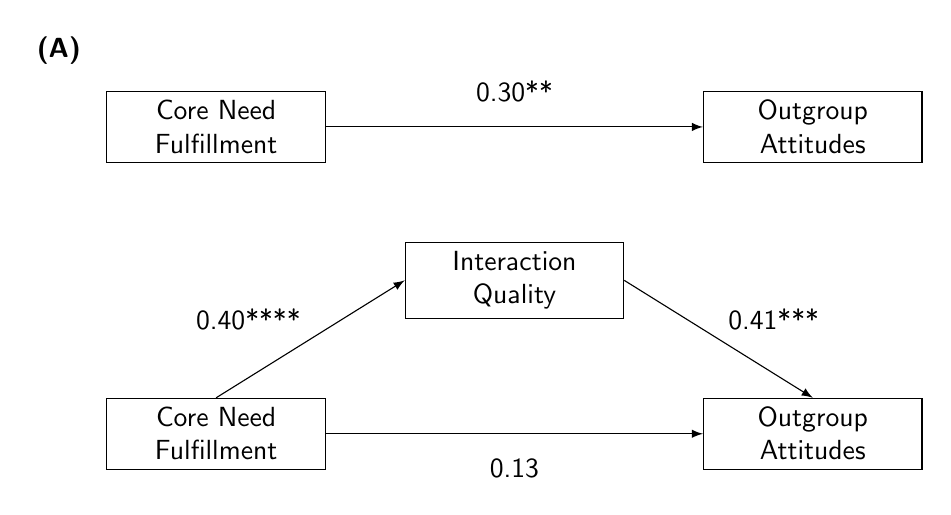
\begin{tikzpicture}[font=\sffamily]
    \node[mynode] (m){Interaction\\Quality};
    \node[mynode,below left=of m](x) {Core Need\\Fulfillment};
    \node[mynode,below right=of m](y) {Outgroup\\Attitudes};
    \node[mynode,above left=of m](xd) {Core Need\\Fulfillment};
    \node[mynode,above right=of m](yd) {Outgroup\\Attitudes};
    \draw[-latex] (xd.east) -- node[above=2mm, align=center] {0.30**} (yd.west);
    \draw[-latex] (x.north) -- node[auto] {0.40****} (m.west);
    \draw[-latex] (m.east) -- node[auto] {0.41***} (y.north);
    \draw[-latex] (x.east) -- node[below=2mm, align=center] {0.13} (y.west);
    \path (xd.north west) ++(-0.2, 6pt) node[above left]{\textbf{(A)}};
\end{tikzpicture}

\vspace{24pt}

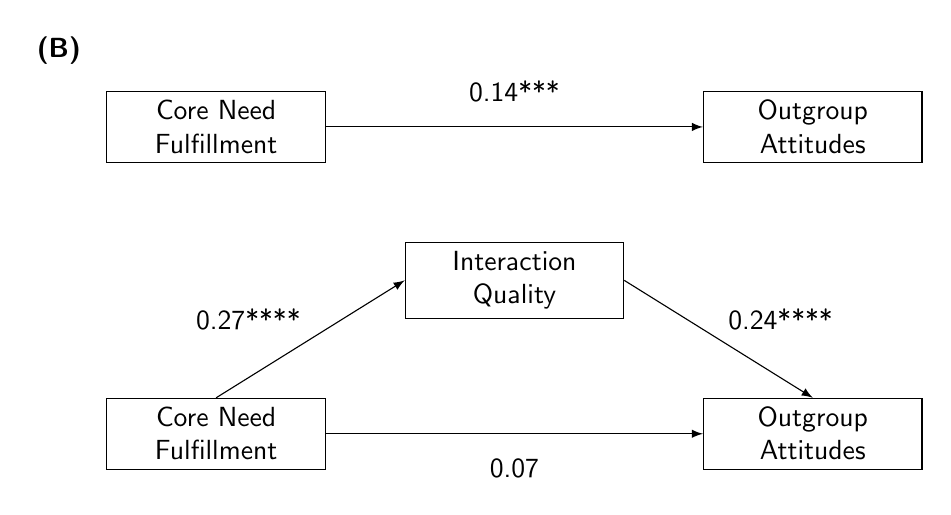
\begin{tikzpicture}[font=\sffamily]
    \node[mynode] (m){Interaction\\Quality};
    \node[mynode,below left=of m](x) {Core Need\\Fulfillment};
    \node[mynode,below right=of m](y) {Outgroup\\Attitudes};
    \node[mynode,above left=of m](xd) {Core Need\\Fulfillment};
    \node[mynode,above right=of m](yd) {Outgroup\\Attitudes};
    \draw[-latex] (xd.east) -- node[above=2mm, align=center] {0.14***} (yd.west);
    \draw[-latex] (x.north) -- node[auto] {0.27****} (m.west);
    \draw[-latex] (m.east) -- node[auto] {0.24****} (y.north);
    \draw[-latex] (x.east) -- node[below=2mm, align=center] {0.07} (y.west);
    \path (xd.north west) ++(-0.2, 6pt) node[above left]{\textbf{(B)}};
\end{tikzpicture}

\vspace{24pt}

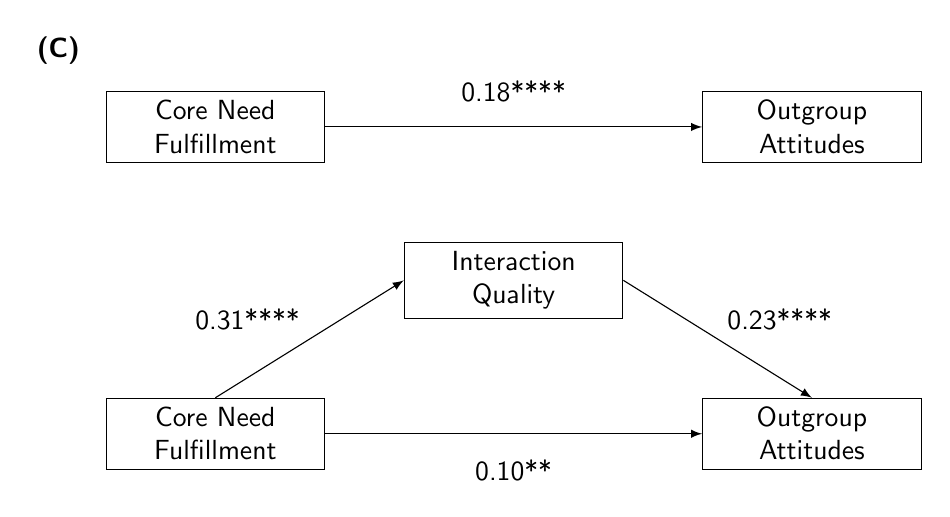
\begin{tikzpicture}[font=\sffamily]
    \node[mynode] (m){Interaction\\Quality};
    \node[mynode,below left=of m](x) {Core Need\\Fulfillment};
    \node[mynode,below right=of m](y) {Outgroup\\Attitudes};
    \node[mynode,above left=of m](xd) {Core Need\\Fulfillment};
    \node[mynode,above right=of m](yd) {Outgroup\\Attitudes};
    \draw[-latex] (xd.east) -- node[above=2mm, align=center] {0.18****} (yd.west);
    \draw[-latex] (x.north) -- node[auto] {0.31****} (m.west);
    \draw[-latex] (m.east) -- node[auto] {0.23****} (y.north);
    \draw[-latex] (x.east) -- node[below=2mm, align=center] {0.10**} (y.west);
    \path (xd.north west) ++(-0.2, 6pt) node[above left]{\textbf{(C)}};
\end{tikzpicture}

  \end{center}
  \caption*{Note: \\
  (A) Study 1; (B) Study 2; (C) Study 3.\\
  General: Path coefficients are standardized regression coefficients. Statistical significance markers are based on the unstandardized regression results (as presented in \tblref{tab:intergroupNeedsTblLong}).\\
  **** p < .0001, *** p < .001, ** p < .01, * p < .05}
\end{figure}

\begin{figure}
  \caption{Contact Hypothesis}
  \label{fig:ContactHypothesis}
  \centering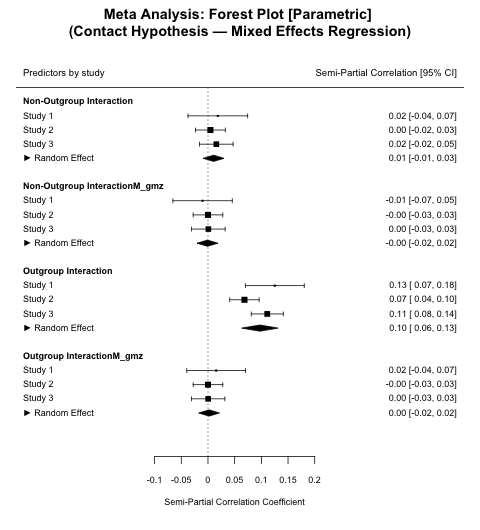
\includegraphics[width=\textwidth]{Figures/forestParametricREMLGeneralLmer.png}
  %\begin{subfigure}{\textwidth}
  %  \caption{}
  %  \centering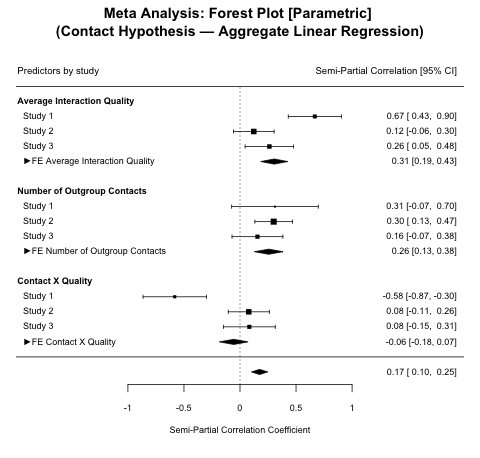
\includegraphics[width=0.75\textwidth]{Figures/forestParametricGeneralLm.png}
  %\end{subfigure}
  %\begin{subfigure}{\textwidth}
  %  \caption{}
  %  \centering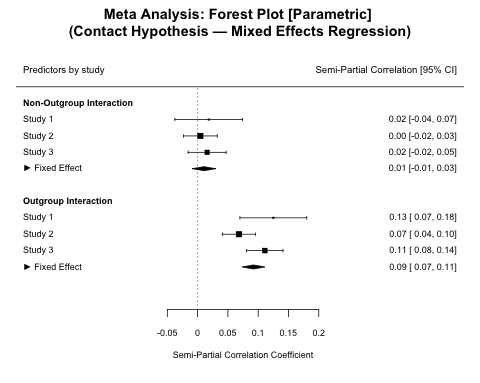
\includegraphics[width=0.75\textwidth]{Figures/forestParametricFEGeneralLmer.png}
  %\end{subfigure}
  \caption*{Note: \\
  Summary of mixed models results of the contemporaneous contact effects.\\
  General: Random effects meta-analytic results are presented for completeness.}
\end{figure}

\begin{figure}
  \caption{Core Need Fulfillment}
  \label{fig:AllportNeedFulfillment}
  \centering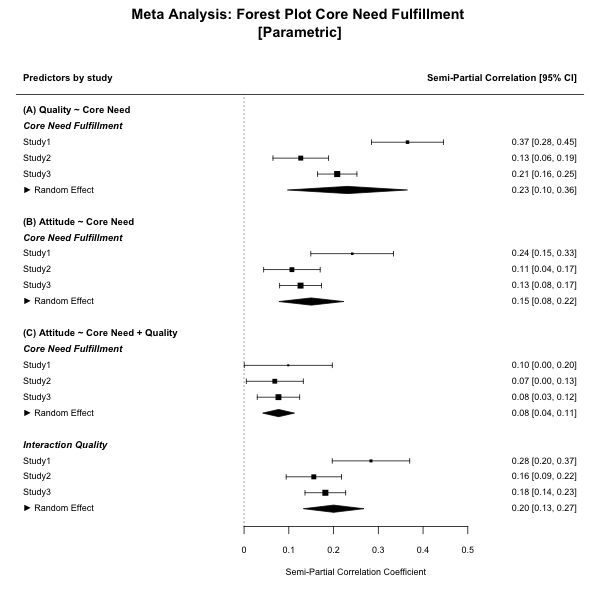
\includegraphics[width=\textwidth]{Figures/forestParametricTheoryComb.png}
  %\begin{subfigure}{\textwidth}
  %  \caption{}
  %  \centering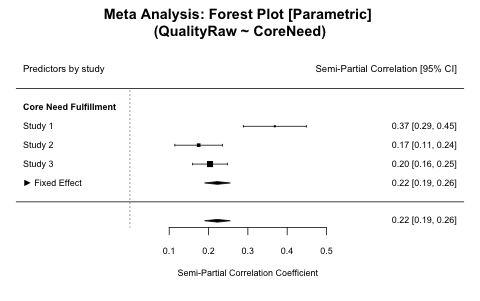
\includegraphics[width=0.6\textwidth]{Figures/forestParametricFETheoryQualityCore.png}
  %\end{subfigure}
  %\begin{subfigure}{\textwidth}
  %  \caption{}
  %  \centering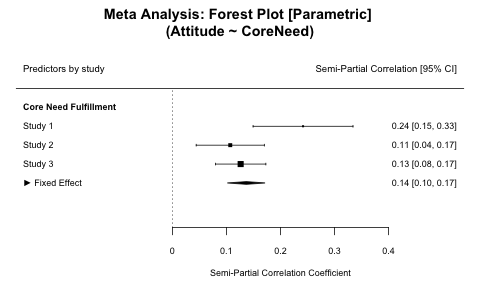
\includegraphics[width=0.6\textwidth]{Figures/forestParametricFETheoryAttitudeCore.png}
  %\end{subfigure}
  %\begin{subfigure}{\textwidth}
  %  \caption{}
  %  \centering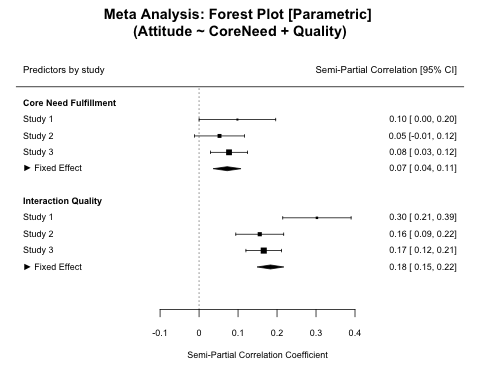
\includegraphics[width=0.6\textwidth]{Figures/forestParametricFETheoryAttitudeCoreQuality.png}
  %\end{subfigure}
  \caption*{Note: \\
  (a) Core Need Fulfillment predicting Interaction Quality.\\
  (b) Core Need Fulfillment predicting Outgroup Attitudes.\\
  (c) Core Need Fulfillment and Interaction Quality predicting Outgroup Attitudes.\\
  General: Random effects meta-analytic results are presented for completeness.}
\end{figure}


\printbibliography

\appendix

\section{Hypotheses and Analysis Plan}
\label{app:AppendixHypotheses}

\newlength{\mdfmar}
\setlength{\mdfmar}{1.5em}
\mdfdefinestyle{mdfhypothesis}{
    innerleftmargin = +1.5\mdfmar, %
    innerrightmargin = +1.5\mdfmar, 
    innertopmargin = +\mdfmar, 
    innerbottommargin = +\mdfmar, 
    skipabove = 12pt
}
\newlength{\subhypskip}
\setlength{\subhypskip}{1.5em}
\newlength{\eqskip}
\setlength{\eqskip}{3.5em}

In this appendix, we present the expanded hypotheses and their associated analysis plan. Given the nested structure of much of our data, we test many of our hypotheses using a multilevel approach, where $y_{ti}$ denotes the response at measurement occasion $t$ ($t = 1, ..., T_i$; level 1) for individual $i$ ($i = 1, ..., n$; level 2). All multilevel assumptions are tested as follows (e.g., for random slopes model with $j$ within-person predictors):

\begin{flalign}
  &\textrm{Level 1 Variance:}\ e_{ti} \sim \mathcal{N}(0,\sigma^2) \\
  &\textrm{Level 2 Variance:}\ \begin{bmatrix} u_{0i}\\ \vdots\\ u_{ji}\end{bmatrix} 
  \sim \mathcal{N}
  \begin{pmatrix}
    \begin{bmatrix} 
      0 \\ 
      \vdots \\
      0
    \end{bmatrix}, 
    \begin{bmatrix} 
      \tau_{00}^2 &  & \\ 
      \vdots & \ddots & \\
      \tau_{j0} & \ldots & \tau_{jj}^2
    \end{bmatrix}
  \end{pmatrix}
\end{flalign}

For our main aims we sequentially focus on four sets of models to test and validate our hypotheses:

\subsection{1. Contact hypothesis in extensive longitudinal data.} 
Within the individual studies, we begin by testing the most basic assumption of the intergroup contact hypothesis that outgroup attitudes should be more positive after outgroup interactions but not after non-outgroup interactions. For this we use multi-level regression analyses, predicting outgroup attitudes from outgroup interaction and non-outgroup interaction dummy variables. We also include the participant means as level two predictors to fully disentangle within- (level 1) and between-participant (level 2) effects of intergroup contact \citep[e.g.,][Section 4.6]{Snijders2012}.

\begin{mdframed}[style=mdfhypothesis]
    \begin{hyp}[H\ref{hyp:contactHyp}] \label{hyp:contactHyp}
        Based on the most general understanding of the contact hypothesis, positive intergroup contacts should be associated with more favorable outgroup attitudes across extensive longitudinal data.
    \end{hyp}
    
    \begin{subhyp}[H\ref{hyp:contactDummyML}] \label{hyp:contactDummyML}
    \addtolength{\leftskip}{\subhypskip}
    Outgroup attitudes should be more positive after an intergroup interaction compared to a non-outgroup interaction.
    \end{subhyp}

    \begin{fleqn}[\eqskip] 
    \begin{equation} \label{eq:ContactDummy}
      \begin{split}
        \textrm{Level 1:} &
          \begin{aligned}[t]
            \ Attitude_{ti} =  &\ \beta_{0i} + \beta_{1i}OutgroupInteraction_{ti} + \\
                               &\ \beta_{2i}NonOutgroupInteraction_{ti} + e_{ti}
          \end{aligned} \\
        \textrm{Level 2:} &
            \begin{aligned}[t]
                \ \beta_{0i} = &\ \gamma_{00} + \gamma_{01}MeanOutgroupInteraction_{i} + \\
                               &\ \gamma_{02}MeanNonOutgroupInteraction_{i} + u_{0i} \\
                  \beta_{1i} = &\ \gamma_{10} + u_{1i} \\
                  \beta_{2i} = &\ \gamma_{20} + u_{2i}
            \end{aligned}
      \end{split} 
    \end{equation}
    \end{fleqn}
\end{mdframed}

% We then seek to investigate intergroup contacts and perceived interaction quality jointly. Notably, however, participants are only able to report their interaction quality perceptions if they had an interaction. This is considered to be structurally missing data and cannot meaningfully be imputed for modeling. To deal with this issue, we mimic the procedure commonly used within the cross-section literature. In particular, we conduct a person-level linear regression by aggregating the number of outgroup interactions participants had, their average interaction quality perceptions, as well as their average outgroup attitudes \citep[for possible alternative approaches see,][]{Enders2011}. To avoid an underpowered analysis, we use the aggregated data from all three studies. 
    
We then seek to test the full contact hypothesis by investigating intergroup contacts and perceived interaction quality jointly. To do so, we conduct a linear regression using person-level aggregated data from all three studies. In particular, we aggregate the number of outgroup interactions participants had, their average interaction quality perceptions, as well as their average outgroup attitudes. This approach has three main benefits: (1) Interaction quality ratings are only available if participants had an interaction, and the aggregation deals with this structural missingness. (2) Using the participant-level data from all three studies, we avoid potential power issues. (3) This analysis mimics the analyses conducted within the cross-section literature, where participants are asked to recall how many interactions they had over a one-month period, how positive these interactions were, and what their general attitudes towards the outgroup are.

\begin{mdframed}[style=mdfhypothesis]
    \begin{subhyp}[H\ref{hyp:contactCor}] \label{hyp:contactCor}
    \addtolength{\leftskip}{\subhypskip}
    Participants with more intergroup interactions should have more favorable outgroup attitudes.
    \end{subhyp}

      \begin{fleqn}[\eqskip] 
        \begin{equation} \label{eq:ContactCor}
            r_{\left(ContactFrequency_{i},\ AverageQuality_{i}\right)} > 0
        \end{equation}
      \end{fleqn}

    \begin{subhyp}[H\ref{hyp:contactQualLM}] \label{hyp:contactQualLM}
    \addtolength{\leftskip}{\subhypskip}
    Participants with more intergroup interactions should have more favorable outgroup attitudes depending on the average interaction quality.
    \end{subhyp}

      \begin{fleqn}[\eqskip] 
        \begin{equation} \label{eq:contactQualLM}
            \begin{split}
              AverageAttitude_{i} = &\ \beta_{0} + \beta_{1}ContactFrequency_{i} + \\
                                    &\ \beta_{2}AverageQuality_{i} +\\
                                    &\ \beta_{3}ContactFrequency_{i} * AverageQuality_{i}
            \end{split}
        \end{equation}
      \end{fleqn}  
      
      We additionally control for the participant's study membership.
\end{mdframed}
Because this analysis uses the data from all three studies, the results of this analysis are presented in the `Robustness, Stability, and Embeddedness across Studies' section.

\subsection{2. Core need fulfillment during intergroup contact.}
The main proposal of this manuscript has been the assertion that the fulfillment of situation core needs during an interaction will be associated with more positive interaction quality perceptions and, ultimately, more positive outgroup attitudes. Thus, for the main set of analyses, we focus on the reported outgroup interactions only. For each study, we will use multi-level regressions to test the main three assertions of our proposal (mirroring the basic steps of a traditional mediation analysis).

\begin{mdframed}[style=mdfhypothesis]
    \begin{hyp}[H\ref{hyp:keyNeed}] \label{hyp:keyNeed}
    Based on our proposal, intergroup interactions with higher situational core need fulfillment should predict more favorable outgroup attitudes due to more positive interaction quality perceptions.
    \end{hyp}
    
    \setcounter{subhyp}{0}
    \begin{subhyp}[H\ref{hyp:keyNeedPred}] \label{hyp:keyNeedPred}
    \addtolength{\leftskip}{\subhypskip}
    Core need fulfillment during outgroup interactions should predict more positive outgroup attitudes.
    \end{subhyp}
    
    \begin{fleqn}[\eqskip]
      \begin{equation} \label{eq:SlopesAttCore}
        \begin{split}
            \textrm{Level 1:} &\ Attitude_{ti} = \beta_{0i} + \beta_{1i}KeyNeedFulfill_{ti} + e_{ti}\\
            \textrm{Level 2:} &\ \beta_{0i} = \gamma_{00} + u_{0i} \\
                              &\ \beta_{1i} = \gamma_{10} + u_{1i}
        \end{split}
      \end{equation}
    \end{fleqn}
    
    \begin{subhyp}[H\ref{hyp:keyNeedQual}] \label{hyp:keyNeedQual}
    \addtolength{\leftskip}{\subhypskip}
    Core need fulfillment during outgroup interactions should also predict higher perceived interaction quality.
    \end{subhyp}
    
    \begin{fleqn}[\eqskip]
      \begin{equation} \label{eq:SlopesQltCore}
        \begin{split}
            \textrm{Level 1:} &\ InteractionQuality_{ti} = \beta_{0i} + \beta_{1i}KeyNeedFulfill_{ti} + e_{ti}\\
            \textrm{Level 2:} &\ \beta_{0i} = \gamma_{00} + u_{0i} \\
                              &\ \beta_{1i} = \gamma_{10} + u_{1i}
        \end{split}
      \end{equation}
    \end{fleqn}
    
    \begin{subhyp}[H\ref{hyp:keyNeedMediation}] \label{hyp:keyNeedMediation}
    \addtolength{\leftskip}{\subhypskip}
    The effect of core need fulfillment on outgroup attitudes should be reduced when considered together with perceived interaction quality.
    \end{subhyp}
    
    \begin{fleqn}[\eqskip]
      \begin{equation} \label{eq:SlopesAttCoreQual}
        \begin{split}
          \textrm{Level 1:} &
            \begin{aligned}[t]
              \ Attitude_{ti} =  &\ \beta_{0i} + \beta_{1i}KeyNeedFulfill_{ti} + \\
                                 &\ \beta_{2i}InteractionQuality_{ti} + e_{ti}
            \end{aligned} \\
          \textrm{Level 2:} &\ \beta_{0i} = \gamma_{00} + u_{0i} \\
                            &\ \beta_{1i} = \gamma_{10} + u_{1i} \\
                            &\ \beta_{2i} = \gamma_{20} + u_{2i}
        \end{split} 
      \end{equation}
    \end{fleqn}
\end{mdframed}

\subsection{3. Allport's conditions in extensive longitudinal data.}
Within the third study, we formally measure all of Allport's optimal contact conditions. We use multi-level regression models to test whether the fulfillment of Allport's conditions in real-life data predicts more positive outgroup attitudes and higher perceived interaction quality, using the same approach as for the core need fulfillment above.

\begin{mdframed}[style=mdfhypothesis]
    \begin{hyp}[H\ref{hyp:Allport}] \label{hyp:Allport}
    Based on Allport's optimal contact conditions, intergroup interactions with equal status, common goals, collaboration, and structural support should predict more favorable outgroup attitudes due to more positive interaction quality perceptions.
    \end{hyp}
    
    \setcounter{subhyp}{0}
    \begin{subhyp}[H\ref{hyp:AttAllport}] \label{hyp:AttAllport}
    \addtolength{\leftskip}{\subhypskip}
    Higher fulfillment of Allport's conditions during outgroup interactions should predict more positive outgroup attitudes.
    \end{subhyp}
    
    \begin{fleqn}[\eqskip]
      \begin{equation} \label{eq:SlopesAttAllport}
        \begin{split}
            \textrm{Level 1:} &\ Attitude_{ti} = \beta_{0i} + \beta_{1i}Allport_{ti} + e_{ti}\\
            \textrm{Level 2:} &\ \beta_{0i} = \gamma_{00} + u_{0i} \\
                              &\ \beta_{1i} = \gamma_{10} + u_{1i}
        \end{split}
      \end{equation}
    \end{fleqn}
    
    \begin{subhyp}[H\ref{hyp:QltAllport}] \label{hyp:QltAllport}
    \addtolength{\leftskip}{\subhypskip}
    Higher fulfillment of Allport's conditions during outgroup interactions should also predict higher perceived interaction quality.
    \end{subhyp}
    
    \begin{fleqn}[\eqskip]
      \begin{equation} \label{eq:SlopesQltAllport}
        \begin{split}
            \textrm{Level 1:} &\ InteractionQuality_{ti} = \beta_{0i} + \beta_{1i}Allport_{ti} + e_{ti}\\
            \textrm{Level 2:} &\ \beta_{0i} = \gamma_{00} + u_{0i} \\
                              &\ \beta_{1i} = \gamma_{10} + u_{1i}
        \end{split}
      \end{equation}
    \end{fleqn}
    
    \begin{subhyp}[H\ref{hyp:AttAllportQual}] \label{hyp:AttAllportQual}
    \addtolength{\leftskip}{\subhypskip}
    The effect of higher fulfillment of Allport's conditions on outgroup attitudes should be reduced when considered together with perceived interaction quality.
    \end{subhyp}
    
    \begin{fleqn}[\eqskip]
      \begin{equation} \label{eq:SlopesAttAllportQual}
        \begin{split}
          \textrm{Level 1:} &
            \begin{aligned}[t]
              \ Attitude_{ti} =  &\ \beta_{0i} + \beta_{1i}Allport_{ti} + \\
                                 &\ \beta_{2i}InteractionQuality_{ti} + e_{ti}
            \end{aligned} \\
          \textrm{Level 2:} &\ \beta_{0i} = \gamma_{00} + u_{0i} \\
                            &\ \beta_{1i} = \gamma_{10} + u_{1i} \\
                            &\ \beta_{2i} = \gamma_{20} + u_{2i}
        \end{split} 
      \end{equation}
    \end{fleqn}
\end{mdframed}

We then compare the effect of Allport's contact conditions with our core need fulfillment by comparing the model fit statistics of the two individual models and by adding both concepts to a joint multi-level regression model, to see whether the two approaches explain the same variance in outgroup attitudes.

\begin{mdframed}[style=mdfhypothesis]
    \begin{hyp}[H\ref{hyp:NeedAllport}] \label{hyp:NeedAllport}
    Based on our proposal, the fulfillment of the core situational need should predict outgroup attitudes at least as well as Allport's conditions.
    \end{hyp}

    \setcounter{subhyp}{0}
    \begin{subhyp}[H\ref{hyp:compModel}] \label{hyp:compModel}
    \addtolength{\leftskip}{\subhypskip}
    The need model (H\ref{hyp:keyNeedPred}) should predict more variance in outgroup attitudes than the model based on Allport's conditions (H\ref{hyp:AttAllport}).
    \end{subhyp}

    \begin{fleqn}[\eqskip] 
        \begin{equation}
            \begin{split}
                AIC_{KeyNeedModel} & < AIC_{AllportModel} \\
                BIC_{KeyNeedModel} & < BIC_{AllportModel}
            \end{split}
        \end{equation}
    \end{fleqn}

    \begin{subhyp}[H\ref{hyp:compTogether}] \label{hyp:compTogether}
    \addtolength{\leftskip}{\subhypskip}
    The  effect of key need fulfillment on outgroup attitudes should  persist even when taking other Allport's conditions into account. Thus, the effect of key need fulfillment on outgroup attitudes should remain strong even after controlling for Allport's conditions.  
    \end{subhyp} 
    
    \begin{fleqn}[\eqskip]
      \begin{equation} \label{eq:SlopesAttCoreAllport}
        \begin{split}
          \textrm{Level 1:} &
            \begin{aligned}[t]
              \ Attitude_{ti} =  &\ \beta_{0i} + \beta_{1i}KeyNeedFulfill_{ti} + \\
                                 &\ \beta_{2i}Allport_{ti} + e_{ti}
            \end{aligned} \\
          \textrm{Level 2:} &\ \beta_{0i} = \gamma_{00} + u_{0i} \\
                            &\ \beta_{1i} = \gamma_{10} + u_{1i} \\
                            &\ \beta_{2i} = \gamma_{20} + u_{2i}
        \end{split} 
      \end{equation}
    \end{fleqn}
\end{mdframed}

\subsection{4. Robustness, stability, and embeddedness across studies}
Within the final set of analyses, we look at the broader picture of our results and leverage the data from all participants to contextualize our results.  

\paragraph{Robustness within studies}
To build further confidence in the effect of core need fulfillment during outgroup interactions, we conduct two additional robustness analyses for each study.

Firstly, to check for the role of alternate psychological needs, we add the fulfillment of self-determination theory needs (i.e., competence, autonomy, and relatedness) to the multi-level regression. We then also compare the model with models that predicts outgroup attitudes from self-determination theory need fulfillments or core need fulfillments only. 

\begin{mdframed}[style=mdfhypothesis]
    \begin{hyp}[H\ref{hyp:keyNeedSDT}] \label{hyp:keyNeedSDT}
    The effect of key need fulfillment on outgroup attitudes should persist even when taking other fundamental psychological needs into account. Thus, the effect of key need fulfillment on outgroup attitudes should remain strong even after controlling for autonomy, competence, and relatedness fulfillment during the interaction (cf., self-determination theory). 
    \end{hyp}
    
    \begin{fleqn}[\eqskip-\subhypskip]
      \begin{equation} \label{eq:SlopesAttCoreSdt}
        \begin{split}
          \textrm{Level 1:} &
            \begin{aligned}[t]
              \ Attitude_{ti} =  &\ \beta_{0i} + \beta_{1i}KeyNeedFulfill_{ti} + \beta_{2i}Autonomy_{ti} + \\
                                 &\ \beta_{3i}Competence_{ti} + \beta_{4i}Relatedness_{ti} + e_{ti}
            \end{aligned} \\
          \textrm{Level 2:} &\ \beta_{0i} = \gamma_{00} + u_{0i} \\
                            &\ \beta_{1i} = \gamma_{10} + u_{1i} \\
                            &\ \beta_{2i} = \gamma_{20} + u_{2i} \\
                            &\ \beta_{3i} = \gamma_{30} + u_{3i} \\
                            &\ \beta_{4i} = \gamma_{40} + u_{4i}
        \end{split} 
      \end{equation}
    \end{fleqn}
\end{mdframed}

To ensure that the core need fulfillment is outgroup contact specific, we return to the full sample of intensive longitudinal measurements within each study and test whether there is an interaction effect of outgroup contact (vs. no outgroup contact) and core need fulfillment. We expect that the effect of core need fulfillment is specific to outgroup interactions and not merely due to a more need-fulfilled life in general.

\begin{mdframed}[style=mdfhypothesis]
    \begin{hyp}[H\ref{hyp:keyNeedContactType}] \label{hyp:keyNeedContactType}
    \addtolength{\leftskip}{1em}
    The effect of key need fulfillment on outgroup attitudes should be specific to intergroup interactions and not be due to need fulfillment in general. Thus, the effect of key need fulfillment on outgroup attitudes should be stronger for intergroup interactions than for ingroup interactions. 
    \end{hyp}
    
    \begin{fleqn}[\eqskip-\subhypskip]
      \begin{equation} \label{eq:SlopesAttCoreXContact}
        \begin{split}
          \textrm{Level 1:} &
            \begin{aligned}[t]
              \ Attitude_{ti} =  &\ \beta_{0i} + \beta_{1i}KeyNeedFulfill_{ti} + \\
                                 &\ \beta_{2i}OutgroupInteraction_{ti} + \\
                                 &\ \beta_{3i}KeyNeedFulfill*OutgroupInteraction_{ti} + e_{ti}
            \end{aligned} \\
          \textrm{Level 2:} &\ \beta_{0i} = \gamma_{00} + u_{0i} \\
                            &\ \beta_{1i} = \gamma_{10} + u_{1i} \\
                            &\ \beta_{2i} = \gamma_{20} + u_{2i} \\
                            &\ \beta_{3i} = \gamma_{30} + u_{3i}
        \end{split} 
      \end{equation}
    \end{fleqn}
\end{mdframed}
The results of the robustness analyses are presented in \appref{app:AppendixRobustness} to allow for a more concise presentation of our main hypotheses in the main text.

\paragraph{Stability across studies}
We assess the stability of our main analyses. We use forest plots (including meta-analytical estimates) to visualize the direction and effect sizes of our three studies.

\begin{mdframed}[style=mdfhypothesis]
    \begin{hyp}[H\ref{hyp:Stability}] \label{hyp:Stability}
    \addtolength{\leftskip}{1em}
    The effects of our main hypotheses and robustness analyses should be consistent across studies.
    \end{hyp}
\end{mdframed}

\paragraph{Embeddedness of code needs}
We, finally, use the qualitative data from the participants' self-identified core needs to contextualize our results. We leverage machine learning to extract a topic model of the free-text entries across the three studies. We describe the extracted topics and themes and compare them to the need contents usually found and measured within the psychological literature. Full methodological details and visualizations are available in Supplemental Material B.

\begin{mdframed}[style=mdfhypothesis]
    \addtolength{\leftskip}{1em}
    \textit{This analysis is data-driven and exploratory. As such, the analysis has no associated hypothesis.}
\end{mdframed}



\section{Robustness Analyses}
\label{app:AppendixRobustness}

In this appendix, we present the two additional robustness analyses that we conducted within each of the three studies. These analyses are specifically designed to check for alternative need models and to check that the effect of situation core need fulfillment is contact-specific. (1) To check for the role of alternate psychological needs, we add the fulfillment of self-determination theory needs (i.e., competence, autonomy, and relatedness) to the multi-level regression. We then also compare the model with models that predicts outgroup attitudes from self-determination theory need fulfillments or core need fulfillments only. (2) To ensure that the core need fulfillment is outgroup contact specific, we return to the full sample of intensive longitudinal measurements within each study and test whether there is an interaction effect of outgroup contact (vs. no outgroup contact) and core need fulfillment. We expect that the effect of core need fulfillment is specific to outgroup interactions and not merely due to a more need-fulfilled life in general.

As with the main analyses, full surveys are available in our OSF
repository \citep{KreienkampMasked2022a} and the full data description
is available in Online Supplementary Material A. Correlations and
descriptive statistics of the included variables are available in
\tblref{tab:descrFullWide} and \tblref{tab:descrOutWide}.

\subsection{Additional Materials}

In addition to the measurement of whether or not participants had an
intergroup interaction and their situational core need fulfillment, we
also measured a set of general psychological needs.

\subsubsection{General Psychological Needs}

In addition to the intergroup contact dummy and situational core need
reported in the main text, we included a common measure of three
self-determination theory needs \citep[see][]{Downie2008}. The
measurement was identical in all three studies. The items were
introduced either by ``\textit{During the interaction:}'' or
``\textit{This morning [/afternoon]:}'' and measured autonomy
(``\textit{I was myself.}''), competence
(``\textit{I felt competent.}''), and relatedness (without intergroup
contact ``\textit{I had a strong need to belong}''; with intergroup
contact: ``\textit{I shared information about myself.}'' and
``\textit{The other(s) shared information about themselves.}''). All
items were rated on a continuous slider scale from very little (-50) to
a great deal (+50).

\subsection{Results}

\subsubsection{Study 1}

To build further confidence in our results, we assessed two additional
models that might offer alternative explanations. First, to ensure that
the effect of core need fulfillment is specific to an actual contact, we
compared the effect to core need fulfillment in situations without an
intergroup contact. For this, we analyzed the generalized situational
core need fulfillment (either during a contact or about the daytime in
general) and tested whether the effect differed during experience
sampling measurements with and without outgroup contacts. We found no
main effect of core need fulfillment (random slopes model; \textit{b} =
-0.10, \textit{t}(1,199) = -2.22, \textit{p} = 0.026,
\textit{95\%CI}{[}-0.18, -0.01{]}) but a significant interaction effect
of core need fulfillment and outgroup contact (\textit{b} = 0.13,
\textit{t}(1,199) = 4.31, \textit{p} \textless{} .001,
\textit{95\%CI}{[}0.07, 0.18{]}; also see \tblref{tab:robustnessTblLong}
and \fgrref{fig:Robustness}). Together with a significant main effect of
having an outgroup contact, this indicates that it is not key need
fulfillment in general --- but only key need fulfillment during an
outgroup contact that predicts more positive outgroup attitudes.

In a final step, we controlled for other fundamental psychological needs
during the contact. We focus on the three commonly considered
self-determination needs (SDT): competence, autonomy, and relatedness.
We find that the core need fulfillment adds significantly above a model
with only the self-determination theory needs (random slopes models;
\(\chi^2\)(6, \textit{N} = 21) = 19.60, \textit{p} = 0.003). We also
find that next to relatedness (\textit{b} = 0.10, \textit{t}(361) =
4.04, \textit{p} \textless{} .001, \textit{95\%CI}{[}0.05, 0.14{]}), the
core need explains the most variance in outgroup attitudes after an
outgroup contact (\textit{b} = 0.09, \textit{t}(361) = 2.23, \textit{p}
= 0.026, \textit{95\%CI}{[}0.01, 0.18{]}). When compared to the model
with only the SDT needs, the core need fulfillment flexibly takes on
some of the explained variance of all three fundamental needs
(competence and autonomy needs turning non-significant; all \textit{b}
\textless{} 0.05, all \textit{p} \textgreater{} 0.544). For full results
see see \tblref{tab:robustnessTblLong} and \fgrref{fig:Robustness}, and
Online Supplementary Material A. There is, thus, considerable evidence
lending confidence to the stability and relevance of psychological need
fulfillment as a predictor of positive outgroup attitudes for natural
intergroup contacts.

\subsubsection{Study 2}

Also for Study 2, we checked for alternative models. First, when
considering generalized situational core need fulfillment together with
whether an intergroup contact took place, we find that there is only a
minuscule main effect of core need fulfillment (random slopes model;
\textit{b} = -0.03, \textit{t}(4,849) = -1.34, \textit{p} = 0.181,
\textit{95\%CI}{[}-0.08, 0.02{]}) but a stronger interaction effect of
core need fulfillment and outgroup contact (\textit{b} = 0.06,
\textit{t}(4,849) = 3.03, \textit{p} = 0.002, \textit{95\%CI}{[}0.02,
0.10{]}). Together with a significant main effect of having an outgroup
contact (\textit{b} = 2.88, \textit{t}(4,849) = 3.71, \textit{p}
\textless{} .001, \textit{95\%CI}{[}1.36, 4.40{]}), this indicates that
it is not key need fulfillment in general --- but key need fulfillment
during an outgroup contact that predicts more positive outgroup
attitudes. This finding is consistent with the results of the previous
study, albeit with a slightly weaker effect (likely because of the large
number of measurements that did not include an outgroup interaction; For
full results see \tblref{tab:robustnessTblLong} and for visual
comparison see \fgrref{fig:Robustness}).

In a final step, we again checked whether during the interaction the
core situational need remains a meaningful predictor even when taking
other fundamental psychological needs into account. We find that the
core need fulfillment adds significantly above a model with only the
self-determination theory needs (random slopes models; \(\chi^2\)(6,
\textit{N} = 108) = 22.90, \textit{p} \textless{} .001). We find that
the core need fulfillment explained the most variance in outgroup
attitudes after an outgroup contact (\textit{b} = 0.08, \textit{t}(823)
= 2.95, \textit{p} = 0.003, \textit{95\%CI}{[}0.03, 0.13{]}). When
compared to the model with only the SDT needs, the core need fulfillment
flexibly takes on some of the explained variance of all of the three
fundamental needs. However, different from the first study, relatedness
(\textit{b} = 0.07, \textit{t}(823) = 4.26, \textit{p} \textless{} .001,
\textit{95\%CI}{[}0.04, 0.10{]}) and autonomy (\textit{b} = 0.02,
\textit{t}(823) = 0.93, \textit{p} = 0.353, \textit{95\%CI}{[}-0.02,
0.08{]}) also predicted positive outgroup attitudes in this larger
sample. For full results see \tblref{tab:robustnessTblLong} and
\fgrref{fig:Robustness}, and Online Supplementary Material A. This means
that also within this second sample, the fulfillment of psychological
needs during intergroup contact remained a key predictor of positive
outgroup attitudes, even when taking into account several alternative
models.

\subsubsection{Study 3}

As with the previous two studies, we checked for alternative models of
the key need fulfillment. First, when considering generalized
situational core need fulfillment together with whether an intergroup
contact took place, we find that there is no significant main effect of
core need fulfillment (random slopes model; \textit{b} = 0.03,
\textit{t}(3,835) = 1.51, \textit{p} = 0.131, \textit{95\%CI}{[}-0.01,
0.06{]}) but a stronger interaction effect of core need fulfillment and
outgroup contact (\textit{b} = 0.17, \textit{t}(3,835) = 7.32,
\textit{p} \textless{} .001, \textit{95\%CI}{[}0.12, 0.21{]}). Together
with a significant main effect of having an outgroup contact (\textit{b}
= 5.41, \textit{t}(3,835) = 6.36, \textit{p} \textless{} .001,
\textit{95\%CI}{[}3.74, 7.08{]}), this indicates that it is not key need
fulfillment in general --- but key need fulfillment during an outgroup
contact that predicts more positive outgroup attitudes. This finding is
consistent with the results of the previous studies.

In a final step, we again checked whether during the interaction the
core situational need remains a meaningful predictor even when taking
other fundamental psychological needs into account. We find that the
core need fulfillment adds additional variance above a model with only
the self-determination theory needs (random slopes models; \(\chi^2\)(6,
\textit{N} = 70) = 100.20, \textit{p} \textless{} .001). We find that
the core need explains the most variance in outgroup attitudes after an
outgroup contact (\textit{b} = 0.15, \textit{t}(1,598) = 3.88,
\textit{p} \textless{} .001, \textit{95\%CI}{[}0.07, 0.22{]}). When
compared to the model with only the SDT needs, the core need fulfillment
flexibly takes on some of the explained variance of all of the three
fundamental needs. However, similar to the previous study, in this large
sample relatedness (\textit{b} = 0.05, \textit{t}(1,598) = 3.31,
\textit{p} \textless{} .001, \textit{95\%CI}{[}0.02, 0.09{]}),
competence (\textit{b} = 0.06, \textit{t}(1,598) = 2.73, \textit{p} =
0.006, \textit{95\%CI}{[}0.02, 0.10{]}) and autonomy (\textit{b} = 0.04,
\textit{t}(1,598) = 2.12, \textit{p} = 0.034, \textit{95\%CI}{[}-0.01,
0.08{]}) each also predicted positive outgroup attitudes independently.
This being said, the regression coefficient for the core need was three
times larger (with all scaling being equal). For full results see
\tblref{tab:robustnessTblLong} and \fgrref{fig:Robustness} as well as
Online Supplementary Material A.


\subsection{Stability and Conclusion}
As with the main analyses, we use a forest plot and the associated meta-analytic estimates to assess the stability of the results across the three studies. The forest plot shows that the core need fulfillment is also consistently outgroup contact specific (\fgrref[-A]{fig:Robustness}) and remains a meaningful predictor of outgroup attitudes even when controlling for traditional psychological need fulfillments (Figure \fgrref[-B]{fig:Robustness}). In sum, we thus find that across all three studies, psychological need fulfillment remained a robust and flexible predictor of positive outgroup attitudes.

\begin{table}
\begin{minipage}[t][\textheight][t]{\textwidth}

\caption{\label{tab:robustnessTblLong}Robustness Analyses}
\centering
\resizebox{\linewidth}{!}{
\begin{tabular}[t]{lcccccccc}
\toprule
\multicolumn{1}{c}{ } & \multicolumn{2}{c}{Overall} & \multicolumn{2}{c}{Study 1} & \multicolumn{2}{c}{Study 2} & \multicolumn{2}{c}{Study 3} \\
\cmidrule(l{3pt}r{3pt}){2-3} \cmidrule(l{3pt}r{3pt}){4-5} \cmidrule(l{3pt}r{3pt}){6-7} \cmidrule(l{3pt}r{3pt}){8-9}
 & $B$ & $\beta$ & $B$ & $\beta$ & $B$ & $\beta$ & $B$ & $\beta$\\
\midrule
\addlinespace[0.3em]
\multicolumn{9}{l}{\textbf{Contact specific}}\\
\hspace{1em}(Intercept) & 65.76** [ 49.86, 72.04] &  & 71.60**** [66.33, 76.86] &  & 68.22**** [64.95, 71.49] &  & 65.17**** [62.00, 68.34] & \\
\hspace{1em}CoreNeed & 0.62 [-13.92, 14.10] & 0.01 [-0.44, 0.45] & 0.09** [ 0.04,  0.14] & 0.21 [0.13, 0.28] & 0.06**** [ 0.04,  0.08] & 0.13 [0.08, 0.17] & 0.11**** [ 0.08,  0.14] & 0.13 [0.09, 0.17]\\
\hspace{1em}OutgroupInteraction & 3.59 [-20.13,  7.99] & -0.60 [-1.74, 0.53] & 1.81* [ 0.25,  3.37] & 0.28 [0.05, 0.50] & 2.88*** [ 1.35,  4.40] & 0.23 [0.16, 0.31] & 5.41**** [ 3.72,  7.10] & 0.37 [0.27, 0.48]\\
\hspace{1em}CoreNeed:OutgroupInteraction & 2.44**** [  0.09,  0.14] & 0.01 [ 0.01, 0.01] & 0.13**** [ 0.07,  0.18] & 0.32 [0.19, 0.45] & 0.06** [ 0.02,  0.10] & 0.14 [0.06, 0.22] & 0.17**** [ 0.12,  0.21] & 0.19 [0.12, 0.26]\\
\hspace{1em}$R^2_{marginal}$ / $R^2_{conditional}$ & 0.000 / 1.000 &  & 0.017 / 0.727 &  & 0.005 / 0.818 &  & 0.037 / 0.712 & \\
\addlinespace[0.3em]
\multicolumn{9}{l}{\textbf{Interaction Intent}}\\
\hspace{1em}(Intercept) & 70.14**** [42.53, 65.97] &  & 71.43**** [65.57, 77.29] &  & 70.40**** [67.36, 73.45] &  & 68.16**** [64.95, 71.36] & \\
\hspace{1em}CoreNeed & 2.87**** [-8.58,  8.95] & 0.02 [-1.22, 1.25] & 0.17** [ 0.06,  0.29] & 0.42 [ 0.26, 0.58] & 0.13*** [ 0.07,  0.20] & 0.25 [ 0.12, 0.37] & 0.19**** [ 0.12,  0.26] & 0.24 [ 0.15, 0.32]\\
\hspace{1em}InteractionAccidental & 0.12 [-9.82,  9.92] & 0.00 [-1.07, 1.07] & 0.03 [ 0.00,  0.06] & 0.13 [ 0.02, 0.24] & 0.01 [-0.02,  0.03] & -0.02 [-0.09, 0.05] & -0.01 [-0.04,  0.01] & -0.02 [-0.08, 0.03]\\
\hspace{1em}CoreNeed:InteractionAccidental & -0.27 [ 0.00,  0.00] & 0.00 [ 0.00, 0.00] & 0.00 [ 0.00,  0.00] & 0.00 [-0.11, 0.11] & 0.00 [ 0.00,  0.00] & -0.01 [-0.08, 0.07] & 0.00 [ 0.00,  0.00] & -0.04 [-0.09, 0.02]\\
\hspace{1em}$R^2_{marginal}$ / $R^2_{conditional}$ & 0.000 / 1.000 &  & 0.135 / NA &  & 0.015 / 0.728 &  & 0.021 / 0.687 & \\
\addlinespace[0.3em]
\multicolumn{9}{l}{\textbf{Well-being Outcome}}\\
\hspace{1em}(Intercept) & 65.25*** [ 28.58, 63.85] &  & 61.34**** [55.56, 67.12] &  & 67.18**** [64.66, 69.70] &  & 63.63**** [60.85, 66.41] & \\
\hspace{1em}CoreNeed & 3.50** [-16.18, 16.62] & 0.01 [-1.33, 1.35] & 0.25** [ 0.10,  0.40] & 0.31 [0.17, 0.46] & 0.10** [ 0.04,  0.16] & 0.17 [0.11, 0.23] & 0.20*** [ 0.11,  0.29] & 0.17 [0.10, 0.25]\\
\hspace{1em}$R^2_{marginal}$ / $R^2_{conditional}$ & 0.000 / 1.000 &  & 0.054 / 0.541 &  & 0.008 / 0.348 &  & 0.017 / 0.375 & \\
\addlinespace[0.3em]
\multicolumn{9}{l}{\textbf{Need Type}}\\
\hspace{1em}(Intercept) & 69.40**** [50.54, 64.07] &  & 73.09**** [66.87, 79.31] &  & 70.37**** [67.24, 73.51] &  & 68.18**** [64.77, 71.60] & \\
\hspace{1em}CoreNeed & 2.27** [ 0.09,  0.21] & 0.01 [-0.82, 0.84] & 0.14* [ 0.03,  0.26] & 0.29 [ 0.12, 0.46] & 0.14** [ 0.06,  0.21] & 0.15 [ 0.04, 0.26] & 0.19*** [ 0.08,  0.29] & 0.18 [ 0.08, 0.29]\\
\hspace{1em}practical need & 0.01 [-4.82,  7.25] & -0.11 [-1.00, 0.78] & -0.04 [-2.76,  2.69] & -0.06 [-0.33, 0.20] & 0.80 [-1.22,  2.82] & 0.17 [ 0.01, 0.32] & -0.99 [-2.85,  0.86] & -0.02 [-0.16, 0.12]\\
\hspace{1em}psychological need & 1.45 [-8.48,  4.45] & -0.13 [-1.11, 0.84] & 1.53 [-3.66,  6.73] & 0.08 [-0.28, 0.43] & 1.50 [-0.98,  3.98] & 0.13 [-0.03, 0.30] & 1.25 [-0.42,  2.93] & 0.10 [-0.04, 0.24]\\
\hspace{1em}CoreNeed:practical need & -0.23 [-0.08,  0.05] & 0.00 [ 0.00, 0.01] & 0.01 [-0.13,  0.15] & -0.12 [-0.36, 0.12] & -0.02 [-0.15,  0.10] & -0.04 [-0.23, 0.14] & -0.05 [-0.18,  0.08] & 0.03 [-0.11, 0.18]\\
\hspace{1em}CoreNeed:psychological need & 0.67 [-0.03,  0.11] & 0.00 [ 0.00, 0.01] & -0.10 [-0.31,  0.11] & -0.02 [-0.33, 0.29] & 0.04 [-0.07,  0.15] & 0.04 [-0.13, 0.21] & 0.04 [-0.11,  0.19] & -0.06 [-0.22, 0.10]\\
\hspace{1em}$R^2_{marginal}$ / $R^2_{conditional}$ & 0.078 / NA &  & 0.046 / NA &  & 0.017 / 0.760 &  & 0.018 / 0.696 & \\
\addlinespace[0.3em]
\multicolumn{9}{l}{\textbf{Specific Psychological Needs}}\\
\hspace{1em}(Intercept) & 70.93** [41.14, 58.40] &  & 71.54**** [65.79, 77.28] &  & 70.75**** [67.59, 73.90] &  & 68.68**** [65.53, 71.82] & \\
\hspace{1em}CoreNeed & 1.88* [-5.45,  5.68] & 0.01 [-1.13, 1.15] & 0.10* [ 0.02,  0.18] & 0.27 [ 0.11, 0.43] & 0.06** [ 0.02,  0.10] & 0.14 [ 0.06, 0.22] & 0.14*** [ 0.07,  0.21] & 0.18 [ 0.09, 0.26]\\
\hspace{1em}Autonomy & 0.78 [-8.61,  8.70] & 0.01 [-1.15, 1.16] & 0.05 [-0.12,  0.23] & 0.12 [-0.02, 0.26] & 0.04 [-0.01,  0.09] & 0.05 [-0.03, 0.13] & 0.04 [ 0.00,  0.08] & 0.05 [-0.03, 0.12]\\
\hspace{1em}Competence & 0.95 [-3.70,  3.78] & 0.00 [-1.11, 1.11] & 0.05 [-0.16,  0.26] & 0.02 [-0.21, 0.25] & 0.05* [ 0.01,  0.10] & 0.06 [-0.03, 0.15] & 0.06* [ 0.01,  0.10] & 0.09 [ 0.02, 0.16]\\
\hspace{1em}Relatednesss & 2.10 [-4.04,  4.19] & 0.01 [-1.20, 1.22] & 0.10*** [ 0.06,  0.14] & 0.29 [ 0.17, 0.41] & 0.06**** [ 0.03,  0.09] & 0.16 [ 0.09, 0.24] & 0.06*** [ 0.02,  0.09] & 0.10 [ 0.02, 0.19]\\
\hspace{1em}$R^2_{marginal}$ / $R^2_{conditional}$ & 0.176 / NA &  & 0.061 / 0.860 &  & 0.025 / 0.747 &  & 0.041 / 0.702 & \\
\bottomrule
\multicolumn{9}{l}{\rule{0pt}{1em}\textit{Note: }}\\
\multicolumn{9}{l}{\rule{0pt}{1em}**** $p$ < .0001, *** $p$ < .001, ** $p$ < .01, * $p$ < .05}\\
\end{tabular}}
\end{minipage}
\end{table}


\begin{figure}
  \caption{Robustness Analyses}
  \label{fig:Robustness}
  \centering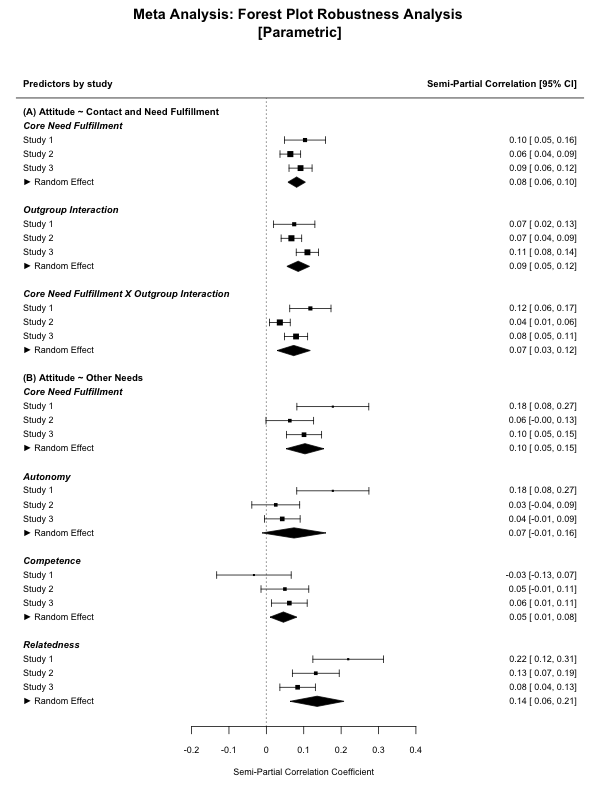
\includegraphics[width=\textwidth]{Figures/forestParametricRobustnessComb.png}
  %\begin{subfigure}{\textwidth}
  %  \caption{}
  %  \centering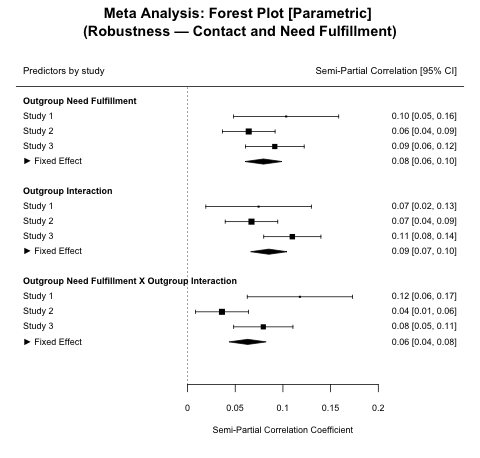
\includegraphics[width=0.65\textwidth]{Figures/forestParametricFERobustContact.png}
  %\end{subfigure}
  %\begin{subfigure}{\textwidth}
  %  \caption{}
  %  \centering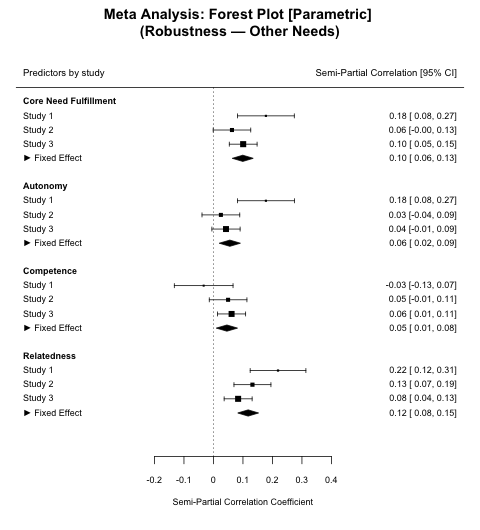
\includegraphics[width=0.65\textwidth]{Figures/forestParametricFERobustSDT.png}
  %\end{subfigure}
  \caption*{Note: \\
  (a) Need Fulfillment and Intergroup Contact predicting Outgroup Attitudes (full sample).\\
  (b) Core Need Fulfillment predicting Outgroup Attitudes while controlling for self-determination theory needs (intergroup contact sample).\\
  General: Random effects meta-analytic results are presented for completeness.}
\end{figure}


\end{document}
